\documentclass[10pt]{beamer}
\usepackage{amsmath,upgreek}
%\usepackage{amsthm}
\usepackage{booktabs,threeparttable}
%\usepackage[capposition=top]{floatrow} % For Figure Notes
\usepackage{mathpazo}
\usepackage{hyperref}
\usepackage{multimedia}
\usepackage{graphicx}
\usepackage{epstopdf}
\usepackage{pause}

%\renewcommand{\rmdefault}{ppl}
\usepackage[scaled=0.88]{helvet}
\makeatletter   % Roman Numbers
\newcommand*{\rom}[1]{\expandafter\@slowromancap\romannumeral #1@}
\makeatother
%\setcounter{MaxMatrixCols}{10}
%TCIDATA{OutputFilter=LATEX.DLL}
%TCIDATA{Version=5.50.0.2890}
%TCIDATA{<META NAME="SaveForMode" CONTENT="1">}
%TCIDATA{BibliographyScheme=Manual}
%TCIDATA{Created=Sunday, May 18, 2008 16:47:28}
%TCIDATA{LastRevised=Tuesday, November 18, 2008 20:57:42}
%TCIDATA{<META NAME="GraphicsSave" CONTENT="32">}
%TCIDATA{<META NAME="DocumentShell" CONTENT="Other Documents\SW\Slides - Beamer">}
%TCIDATA{CSTFile=beamer.cst}

\newcommand{\E}{\mathbb{E}}
\newcommand{\e}{\mathrm{e}}
\newcommand{\I}{\mathbb{I}}
\DeclareMathOperator*{\argmax}{argmax}
\DeclareMathOperator*{\plim}{plim}
\renewcommand{\vec}[1]{\ensuremath{\mathbf{#1}}}
\newcommand{\gvec}[1]{{\boldsymbol{#1}}}
\renewcommand{\qedsymbol}{$\blacksquare$}
\newenvironment{stepenumerate}{\begin{enumerate}[<+->]}{\end{enumerate}}
\newenvironment{stepitemize}{\begin{itemize}[<+->]}{\end{itemize} }
\newenvironment{stepenumeratewithalert}{\begin{enumerate}[<+-| alert@+>]}{\end{enumerate}}
\newenvironment{stepitemizewithalert}{\begin{itemize}[<+-| alert@+>]}{\end{itemize} }
\newtheorem{proposition}{Proposition}[section]
\newcommand{\bcode}[1]{\texttt{{\color{blue}{#1}}}}
\newcommand{\rcode}[1]{\texttt{{\color{red}{#1}}}}
\newcommand{\rtext}[1]{{\color{red}{#1}}}
\newcommand{\btext}[1]{{\color{blue}{#1}}}
\newcommand{\code}{\texttt}
\definecolor{purpledef}{RGB}{51,51,178}

\setbeamertemplate{caption}[numbered]
%\usefonttheme{serif}
%\usetheme{Madrid}
%\usetheme{Warsaw}
%\usetheme{JuanLesPins}
%\usetheme{Berlin}
%\usetheme{Boadilla}
%\usetheme{default}

\makeatletter
\setbeamertemplate{footline}
{
  \leavevmode%
  \hbox{%
  \begin{beamercolorbox}[wd=.333333\paperwidth,ht=2.25ex,dp=1ex,center]{author in head/foot}%
    \usebeamerfont{author in head/foot}\insertshortauthor
  \end{beamercolorbox}%
  \begin{beamercolorbox}[wd=.333333\paperwidth,ht=2.25ex,dp=1ex,center]{title in head/foot}%
    \usebeamerfont{title in head/foot}\insertshorttitle
  \end{beamercolorbox}%
  \begin{beamercolorbox}[wd=.333333\paperwidth,ht=2.25ex,dp=1ex,right]{date in head/foot}%
    \usebeamerfont{date in head/foot}\insertshortdate{}\hspace*{2em}
    \insertframenumber{} / \inserttotalframenumber\hspace*{2ex}
  \end{beamercolorbox}}%
  \vskip0pt%
}
\makeatother

\title[Firm Size and Industrial Pollution]{\large The Size Distribution of Firms and Industrial Water Pollution \\ A Quantitative Analysis of China}
\author[Qi, Tang and Xi]{{Ji Qi} \inst{\star} \and {Xin Tang} \inst{\dagger} \and {Xican Xi} \inst{\ddagger}}
\institute[MEP \& IMF \& FDU]{
    \inst{\star} {Chinese Academy for Environmental Planning} \and
    \inst{\dagger} {International Monetary Fund} \and
    \inst{\ddagger} {Fudan University}}
\date[IMF (RES) Fall 2019]{\footnotesize{\today} \\ \scriptsize{The views expressed here are those of the authors and do not necessarily reflect the views of the CAEP and the IMF.}}

\begin{document}

\frame{\titlepage}

\section{Introduction}

\begin{frame}
\frametitle{Motivation}
\begin{itemize}
\itemsep=0.15in
    \item
    Rapid economic growth in China is paired with severe environmental consequences.
    \begin{itemize}
        \item
        Is pollution an inevitable consequence of growth or exacerbated by policy distortions and/or market inefficiencies?
    \end{itemize}
    \item
    We argue that misallocation across firms reduces output and amplifies industrial pollution by distorting the firm size distribution.
    \item
    \textit{\color{blue}Policy Implications}:
    \begin{itemize}
        \item
        Reducing the distortions firms face increases output while reducing pollution.
        \item
        Environmental regulations could amplify existing market distortions.
    \end{itemize}
    \item
    We believe that the findings of our paper could be generalized to
    \begin{itemize}
        \item air and solid waste pollution;
        \item the agricultural sector;
        \item other developing countries.
    \end{itemize}
\end{itemize}
\end{frame}

\begin{frame}
\frametitle{Intuition}
\begin{itemize}
\itemsep=0.15in
    \item
    \textit{\color{blue}Hypothesis}: Distortions $\rightarrow$ Size Distribution $\rightarrow$ Industrial Pollution.
    \begin{itemize}
    \itemsep=0.10in
        \item
        Larger firms have lower pollution intensity because they use cleaner production and treatment technologies.
        \item
        Distortions limit the expansion of productive firms in China.
        \item
        Compared to an economy with fewer distortions (e.g., the U.S.), less productive firms with higher pollution intensity are active.
        \item
        As a result, aggregate output is lower, but industrial pollution is higher.
    \end{itemize}
    \item
    Technique effect dominates scale effect.
    \item
    \textit{\color{blue}Significance}: Growth and environmental protection are not necessarily a trade-off.
\end{itemize}
\end{frame}

\begin{frame}
\frametitle{Overview of Results}
\begin{itemize}
\itemsep=0.15in
    \item
    Empirical Evidence:
    \begin{itemize}
        \item
        Large firms have lower pollution intensity.
        \item
        Correlated distortions limit the expansion of large firms.
    \end{itemize}
    \item
    Model:
    \begin{itemize}
        \item
        Two sectors (polluting and non-polluting);
        \item
        Firms heterogeneous in productivity, pollution intensity and correlated distortions;
        \item
        Endogenous treatment technology choice with imperfect regulations.
    \end{itemize}
    \item
    Qualitative Results:
    \begin{itemize}
        \item
        Correlated distortions discourage technology adoption.
        \item
        When would technique effect dominates scale effect.
    \end{itemize}
    \item
    Quantitative Exercises:
        \begin{itemize}
        \item
        Removing distortions: $Y \uparrow $ 30\%, $E \downarrow $ 20\%.
        \item
        Strengthening regulations: $Y = $, $E \downarrow $ 15\%.
        \end{itemize}
\end{itemize}
\end{frame}

\begin{frame}
\frametitle{Related Literature}
\begin{itemize}
\itemsep=0.15in
    \item
    Misallocation:
    \begin{itemize}
        \item
        Restuccia and Rogerson (2008), Guner et al. (2008), Hsieh and Klenow (2009).
        \item
        We consider both the output and pollution.
    \end{itemize}
    \item
    Economic Growth and Environment:
    \begin{itemize}
        \item
        Grossman and Krueger (1993, 1995), Copeland and Taylor (2004), Levinson (2009).
        \item
        Cherniwchan et al. (2017), Shapiro and Walker (2018).
        \item
        We focus on a theoretical interpretation behind the scale and technique effects.
    \end{itemize}
    \item
    Technology Adoption in Developing Countries:
    \begin{itemize}
        \item
        Parente and Prescott (1994, 1999), Bustos (2011), Acemoglu et al. (2012).
        \item
        We study the role of size and misallocation.
    \end{itemize}
    \item
    {\color{black}Industrial Pollution in China}��
    \begin{itemize}
        \item
        Jiang et al. (2014), Kahn et al. (2015), Cai et al. (2016), Jia (2017).
        \item
        We emphasize the role of distortions and size distribution.
    \end{itemize}
\end{itemize}
\end{frame}

\begin{frame}
\frametitle{Outline}
\begin{itemize}
\itemsep=0.15in
    \item
    Empirical Evidence:
    \begin{itemize}
        \item Data
        \item Fact: Pollution Intensity
        \item Fact: Employment Distribution
    \end{itemize}
    \item
    The Model:
    \begin{itemize}
        \item Measuring Distortions
        \item Analytical Properties
    \end{itemize}
    \item
    Quantitative Results:
    \begin{itemize}
        \item Removing Distortions
        \item Tightening Regulations
    \end{itemize}
\end{itemize}
\end{frame}

\section{Empirical Evidence}

\begin{frame}
\begin{center}
\LARGE{1. Empirical Evidence}
\end{center}
\end{frame}

\subsection{Data Sources}

\begin{frame}
\frametitle{Data}
\framesubtitle{Data Sources}
\begin{itemize}
\itemsep=0.15in
    \item
    National General Survey of Pollution Sources (2007)
    \begin{itemize}
    \item
    Firm sales, emission, and treatment equipment.
    \end{itemize}
    \item
    China National Economic Census (2004)
    \begin{itemize}
    \item
    Firm sales, employment, labor compensation, and capital stock.
    \end{itemize}
    \item
    Statistics of U.S. Business (2004)
    \begin{itemize}
    \item
    Firm size distribution in the U.S.
    \end{itemize}
\end{itemize}
\end{frame}

\begin{frame}[label=datasource]
\frametitle{Data}
\framesubtitle{Measurement}
\begin{itemize}
\itemsep=0.15in
    \item
    We use Chemical Oxygen Demand (COD) as the main measure.
    \begin{itemize}
    \itemsep=0.10in
    \item More than 70\% of firms in our sample have positive COD emissions.
    \item COD emission is highly correlated with those of other pollutants.
    \item In the Paper industry, $\text{corr}(\text{NH}_4^+,\text{COD}) = 0.82$, and $\text{corr}(\text{BOD},\text{COD}) = 0.94$.
    \end{itemize}
    \item
    We focus on the 5 most polluting industries.
    \begin{itemize}
    \item They account for 77\% of total COD emission in China.
    \end{itemize}
    \item
    We focus on the key sources.
    \begin{itemize}
        \item For the polluting industries, they account for 90\% of the emissions, and 80\% of the production.
    \end{itemize}
\end{itemize}
\hyperlink{coddef}{\beamergotobutton{COD Definition}}
\hyperlink{pollutants}{\beamergotobutton{Pollutants}}
\end{frame}

\begin{frame}[label=codquartile]
\frametitle{Firm Size and Pollution Intensity}
\framesubtitle{Scatter Plots}
\begin{itemize}
\itemsep=0.15in
    \item
    Emission intensity = emission/sales.
\end{itemize}
\begin{figure}[htb]
\begin{center}
    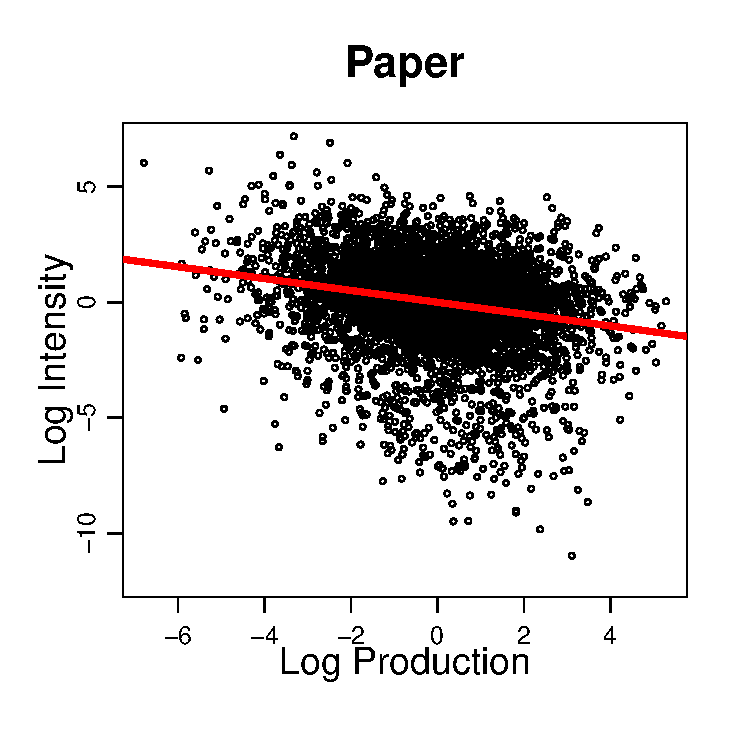
\includegraphics[width=0.45\textwidth]{./Figures/paper_ez.pdf}
    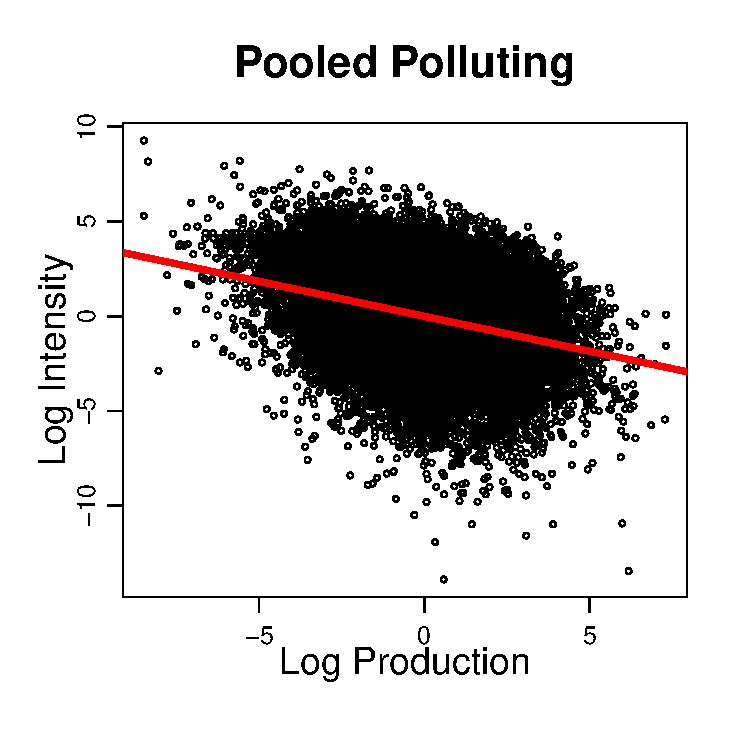
\includegraphics[width=0.45\textwidth]{./Figures/pooled_intensity_size.pdf}
\end{center}
\end{figure}
\hyperlink{codscatter}{\beamergotobutton{Scatter by Industries}}
\end{frame}

\begin{frame}[label=codreg]
\frametitle{Firm Size and Pollution Intensity}
\framesubtitle{Regression Results}
\begin{itemize}
\itemsep=0.15in
    \item
    Regression Specification:
    \begin{align*}
        \log (\text{COD}_i) = &\underset{(0.17)}{-3.75} + \underset{(0.01)}{0.63} \times \log (\text{Output}_i) + \mathbf{X}_i\gvec{\upgamma} + \varepsilon_i, \\
        & N = 29,019, R^2 = 0.41.
    \end{align*}
    \item
    $\mathbf{X}_i$ controls for sectors, provinces, and ownership rights.
    \begin{itemize}
        \item Pollution intensity does \rtext{not} vary systematically with \btext{ownership rights}.
    \end{itemize}
    \item
    As sales rise by 1\%, emission intensity drops by $(1-0.63) = 0.37\%$.
\end{itemize}
\end{frame}

\begin{frame}[label=treatment1]
\frametitle{Treatment Technologies and Firm Size}
\begin{itemize}
\itemsep=0.15in
    \item
    For the Paper industry:
    \begin{itemize}
    \item
    Treatment efficiency ($1 - \text{COD Emitted}/\text{COD Generated}$):
    \end{itemize}
\end{itemize}

\begin{table}[t]
    \small
    \centering
    \begin{threeparttable}
    \begin{tabular}{p{80pt}p{75pt}p{50pt}p{50pt}}
        \hline \hline
        Technology          & Physical          & Chemical      & Biological \\
        \midrule
        Adoption Rate       & 26\%              & 34\%          & 39\%    \\
        Mean Efficiency     & 63\%              & 75\%          & 81\%    \\
        \midrule
        Median Costs        & 100 (Normalized)  & 308           & 923     \\
        Median Sales        & 100 (Normalized)  & 219           & 500     \\
        \bottomrule
    \end{tabular}
    \end{threeparttable}
\end{table}

\begin{itemize}
    \item
    A linear probability model of biological equipment adoption on log-output:
    \begin{equation*}
        y_i = \underset{(0.04)}{0.23} + \underset{(0.001)}{0.05} \times \log (\text{Output}_i) + \mathbf{X}_i\gvec{\upgamma} + \epsilon_i.
    \end{equation*}
\end{itemize}
\hyperlink{treatment2}{\beamergotobutton{Examples}}
\hyperlink{treattech2}{\beamergotobutton{Additional Tech Specs}}
\end{frame}

\begin{frame}[label=producttech]
%\small
\frametitle{Production Technologies and Firm Size}
\framesubtitle{Regression Results}
\begin{itemize}
\itemsep=0.15in
    \item
    Large firms also {\color{black}generate} less pollution conditional on treatment technology.
    \item
    Regression Specifications:
    \begin{align*}
        \text{Physical:}   \quad \log (\text{COD}_i) &= \underset{(0.40)}{-3.50} + \underset{(0.01)}{0.58} \times \log (\text{Sales}_i) + \mathbf{X}_i\gvec{\upgamma} + \epsilon_i, \\
        \text{Chemical:}   \quad \log (\text{COD}_i) &= \underset{(0.49)}{-4.59} + \underset{(0.01)}{0.77} \times \log (\text{Sales}_i) + \mathbf{X}_i\gvec{\upgamma} + \epsilon_i, \\
        \text{Biological:} \quad \log (\text{COD}_i) &= \underset{(0.20)}{-4.37} + \underset{(0.01)}{0.67} \times \log (\text{Sales}_i) + \mathbf{X}_i\gvec{\upgamma} + \epsilon_i.
    \end{align*}
\end{itemize}
%\hyperlink{treattech}{\beamergotobutton{Treatment Technology Choice}}
\end{frame}

\begin{frame}[label=producttech2]
\frametitle{Production Technologies and Firm Size}
\framesubtitle{Possible Interpretations}
\begin{itemize}
\itemsep=0.15in
    \item
    An example from the \textit{Handbook of Emission Coefficients} by the \textit{Chinese Academy of Sciences}:
    \begin{itemize}
    \item Two technologies in paper pulp manufacturing use different inputs: {\color{black}bagasse} and {\color{black}wood}.
    \item {\color{black}Bagasse} is used mostly by firms with annual production of {\color{red}less} than 100 k-tons with COD generation of 140--180 kg per ton.
    \item {\color{black}Wood} is used mostly by firms with annual production {\color{red}more} than 100 k-tons with COD generation of 30--55 kg per ton.
    \end{itemize}
    \item
    It could also be that more productive firms simply use less input (Bloom et al. 2010).
    \item
    We capture such decrease in intensity in a reduced-form way.
\end{itemize}
\end{frame}

\begin{frame}[label=esdistall]
\frametitle{Firm Size Distributions}
\begin{figure}[htb]
\begin{center}
    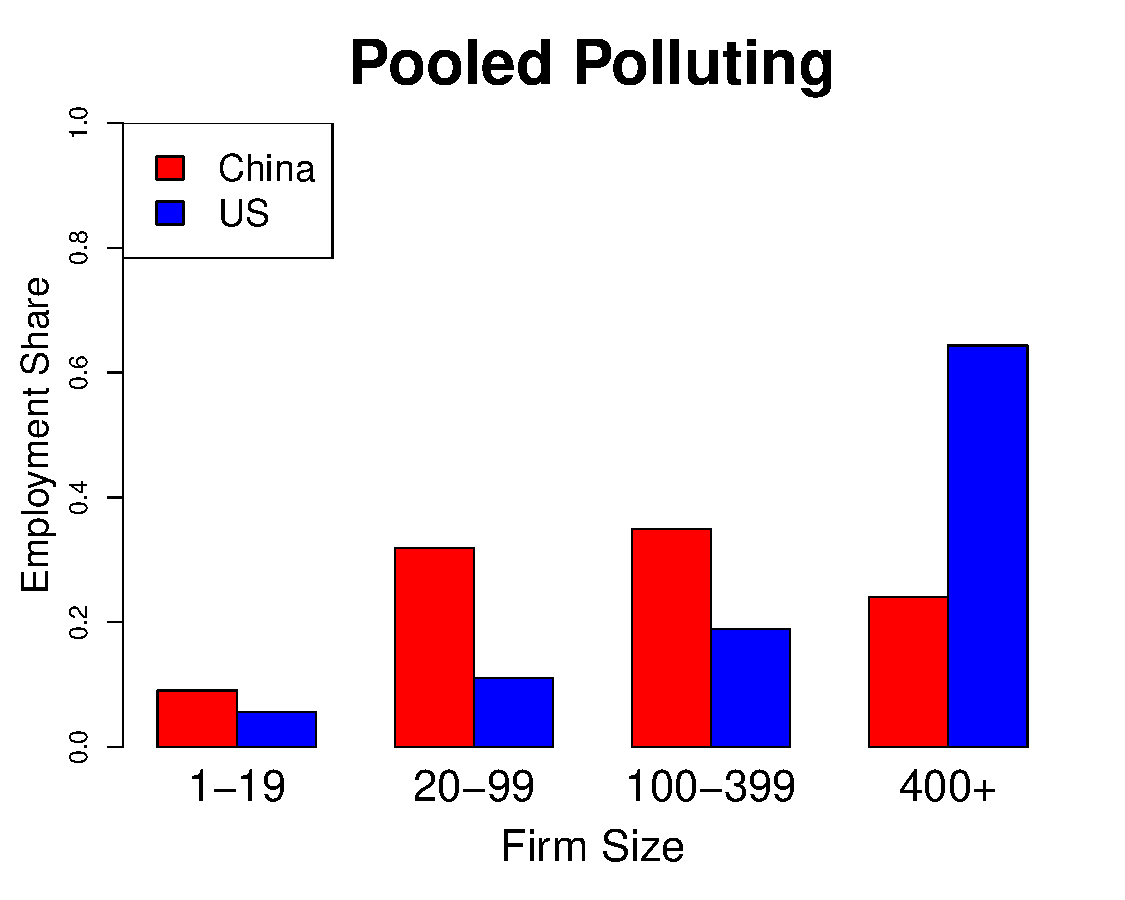
\includegraphics[width=0.45\textwidth]{./Figures/poolES_R_1.pdf}
    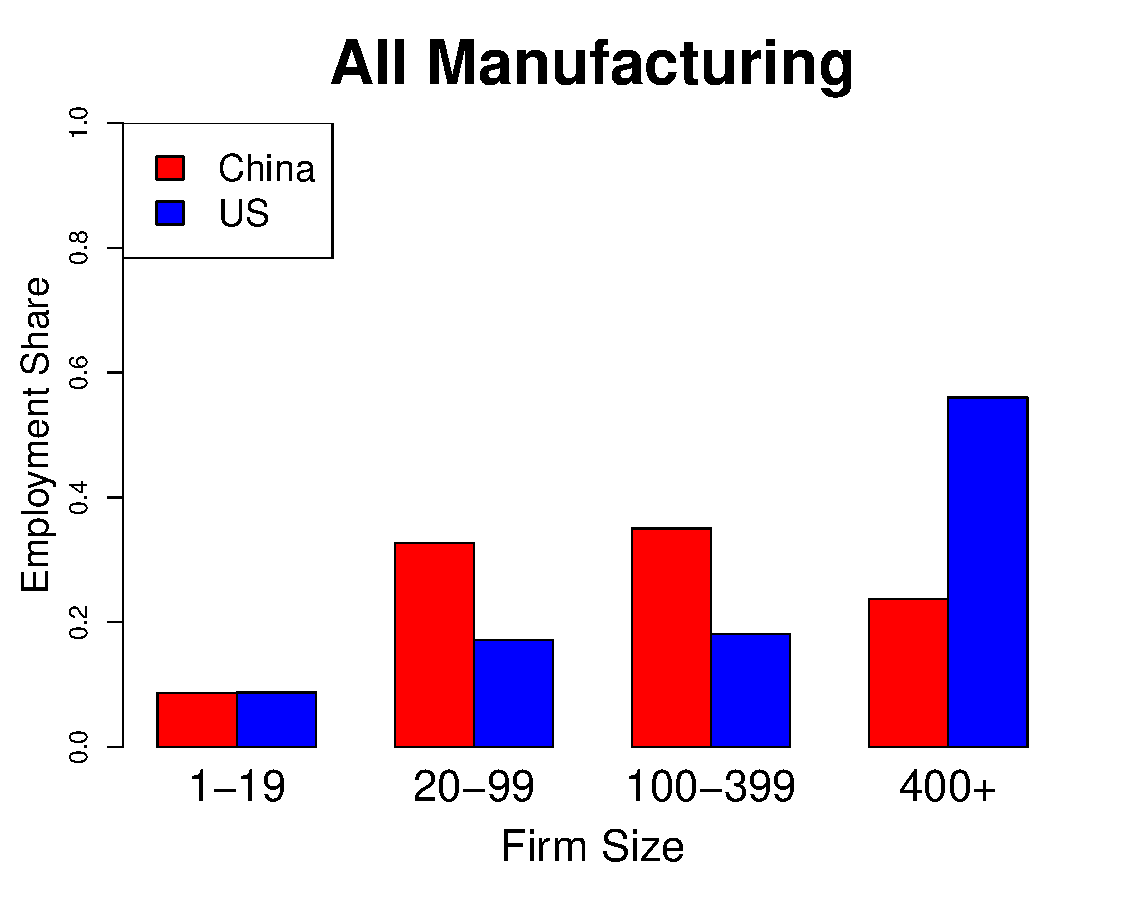
\includegraphics[width=0.45\textwidth]{./Figures/allES_R_1.pdf}
\end{center}
\end{figure}
\hyperlink{esdist}{\beamergotobutton{By Industry}}
\end{frame}

\begin{frame}[label=accounting]
\frametitle{Accounting Exercise}
\begin{itemize}
\itemsep=0.15in
    \item
    {\color{blue}Question:} How will the {\color{black}average pollution intensity} change if the {\color{black}size distribution} is mechanically changed to that in the U.S.?
    \begin{itemize}
    \itemsep=0.10in
        \item
        Production level is fixed.
        \item
        The relation between pollution intensity and firm size in China is used.
        \item
        It captures the \textit{Technique} effect while holding the \textit{Scale} effect constant.
    \end{itemize}
    \item
    {\color{blue}Answer:} Average pollution intensity would drop by 33\%.
\end{itemize}
\hyperlink{accountingrbst}{\beamergotobutton{Robustness}}
\end{frame}

\section{The Model}

\begin{frame}
\begin{center}
\LARGE{2. The Model}
\end{center}
\end{frame}

%\begin{frame}
%\frametitle{Why Are We \textit{Not} Done Yet?}
%The accounting exercise has several limitations:
%\begin{itemize}
%    \item
%    Aggregate output is fixed.
%    \item
%    Firm size distribution is mechanically changed to that in the U.S.
%    \item
%    The firm size and emission intensity relationship is taken as invariant.
%\end{itemize}
%\end{frame}

\begin{frame}
%\frametitle{We Need a Model}
\frametitle{Why Are We \textit{Not} Done Yet?}
\begin{itemize}
\itemsep=0.15in
    \item
    The accounting exercise has several limitations:
    \begin{itemize}
    \itemsep=0.10in
        \item
        Only the polluting sector is considered.
        \item
        Aggregate output is fixed.
        \item
        Firm size distribution is mechanically changed to that in the U.S.
        \item
        The firm size and pollution intensity relationship is taken as invariant.
    \end{itemize}
    %\pause
    \item
    To better evaluate the environmental consequences of distortions to firm size, we need a model:
    \begin{itemize}
    \itemsep=0.10in
        \item
        features two sectors;
        \item
        where distortions affect both aggregate output and pollution;
        \item
        which reveals why firm size is distorted and how it will be changed;
        \item
        and which features treatment technology choice.
    \end{itemize}
\end{itemize}
\end{frame}

\subsection{Setup}
\begin{frame}
\frametitle{Overview of the Model}
\begin{itemize}
\itemsep=0.15in
    \item
    A two-sector model with perfect substitution between products.
    \item
    Each sector features a Lucas (1978) span-of-control model.
    \item
    Firms differ in productivity and pollution intensity.
    \item
    Firms can use treatment equipment to reduce emissions.
    \begin{itemize}
    \item The cost of treatment equipment is independent of firm size.
    \item There are penalties for not using clean technology.
    \end{itemize}
    \item
    Correlated distortions that increase with firm size (Restuccia and Rogerson, 2008).
    \begin{itemize}
    \item Domestic local protectionism, size-dependent tax treatments, etc.
    \end{itemize}
    \item
    {\color{black}Steady state} analysis.
\end{itemize}
\end{frame}

\begin{frame}
\frametitle{Household}
\begin{itemize}
\itemsep=0.15in
    \item
    A representative household with a continuum of members:
    \begin{equation*}
        \sum_{t=0}^{\infty} \beta^t U(C_t).
    \end{equation*}
    \item
    Each member is endowed with $z$ units of \btext{sector-specific} managerial talent.
    \begin{itemize}
        \item The CDFs are $G^c(z)$ and $G^d(z)$ with a common support $Z \triangleq [0,\overline{z}]$;
        \item $z$ is fixed once drawn.
        \item A fraction $\mu$ of members possess talent in the \btext{polluting} sector.
    \end{itemize}
    \item
    Members can only become entrepreneurs in their designated sector, but are free to enter both sectors as worker.
    \item
    The household owns all firms and capital in the economy.
\end{itemize}
\end{frame}

\begin{frame}[label=firmset]
\frametitle{Firms}
\framesubtitle{Non-polluting Sector}
\begin{itemize}
\itemsep=0.15in
    \item
    The production function is the same in both sectors:
    \begin{equation*}
        y = F(z,k,l) = z^{1-\gamma}(k^{\alpha}l^{1-\alpha})^{\gamma},
    \end{equation*}
    where $0<\gamma<1$ is the span-of-control parameter.
    \item
    Firms in the non-polluting sector do not discharge pollutants and are not subject to environmental regulations.
\end{itemize}
\end{frame}

\begin{frame}[label=treattech]
\frametitle{Firms}
\framesubtitle{Polluting Sector: Clean Technology and Regulations}
\begin{itemize}
\itemsep=0.15in
    \item
    Treatment Technologies:
    \begin{itemize}
    \itemsep=0.10in
        \item
        Emissions $e$ are by-product of production:
        \begin{equation*}
            \log \left(\frac{e}{y}\right) = \psi_0^j + \psi_1^j \log y, \quad j = 0,1,
        \end{equation*}
        where $j=1$ indicates clean technology and $\psi_1^j < 0$.
        \item
        Clean technology requires fixed installation costs $k_E$.
    \end{itemize}
    %\pause
    \item
    Regulations:
    \begin{itemize}
    \itemsep=0.10in
        \item
        If a firm using dirty technology is inspected, a fraction $\xi$ of its total profits $\pi(z)$ is confiscated.
    \end{itemize}
        %\pause
    \begin{itemize}
        \item Confiscated profits are rebated back to household as {\color{black}lump-sum} transfers.
    \end{itemize}
\end{itemize}
%\hyperlink{producttech}{\beamergotobutton{Evidence on $\psi_1^{i}$}}
\end{frame}

\begin{frame}[label=firmset]
\frametitle{Which Distortion Matters?}
\framesubtitle{Identification Assumption}
\begin{itemize}
\itemsep=0.15in
    \item
    We use the variations in average factor products to measure these wedges (Hsieh and Klenow, 2009).
    \item
    Let {\color{blue}$\tau_{z_i}, \tau_{k_i}$} and {\color{blue}$\tau_{l_i}$} be the wedges firm $i$ faces on the product, capital and labor market, the problem of firm $i$ is
    \begin{equation*}
      \pi_i = \max_{k_i,l_i} \left\{ (1-\tau_{z_i}) z_i^{1-\gamma} (k_i^{\alpha} l_i^{1-\alpha})^{\gamma} - (1+\tau_{k_i})Rk_i - (1+\tau_{l_i})W l_i \right\}.
    \end{equation*}
    \item
    Assuming $\tau_{l_i} = 0$:
    \begin{align*}
        \frac{y_i}{l_i} &= \frac{W}{(1-\alpha) \gamma (1-\tau_{z_i})} \varpropto \frac{1}{1-\tau_{z_i}}, \\
        \frac{k_i}{l_i} &= \frac{\alpha}{1-\alpha} \cdot \frac{W}{(1+\tau_{k_i})R} \varpropto \frac{1}{1+\tau_{k_i}}.
    \end{align*}
\end{itemize}
\end{frame}

\begin{frame}[label=arp]
\frametitle{Which Distortion Matters?}
\framesubtitle{Data}
\begin{itemize}
    \item
    Using the China National Economic Census, we find:
    \makebox[\linewidth]{
    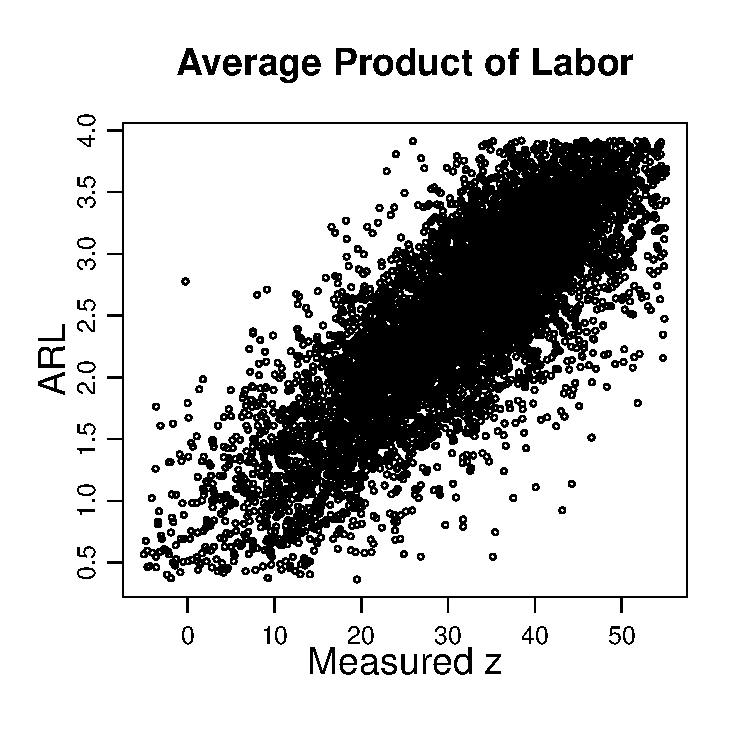
\includegraphics[width=0.33\paperwidth,height=0.4\paperheight]{D:/PaperDrafts/Pollution/R_Implementation/arpl_1.pdf}
    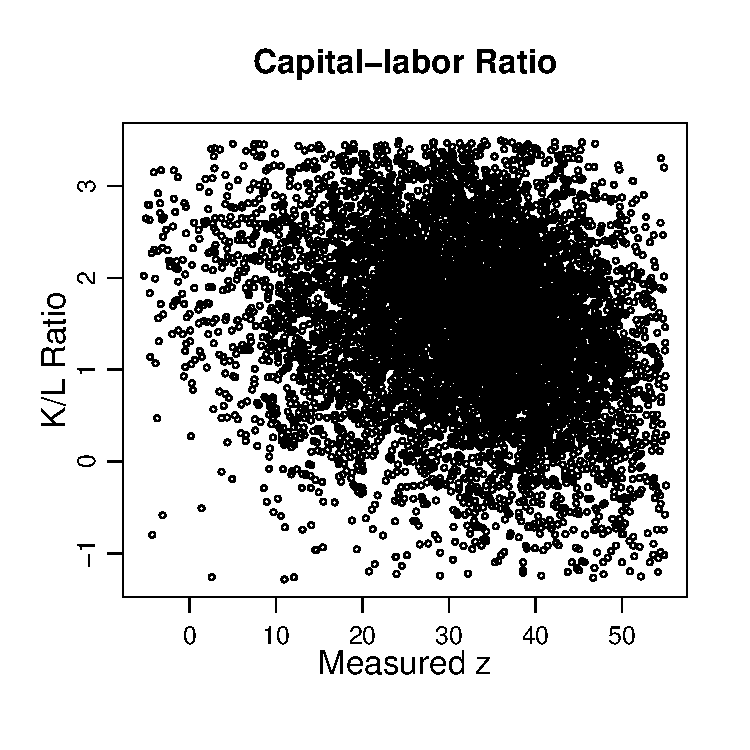
\includegraphics[width=0.33\paperwidth,height=0.4\paperheight]{D:/PaperDrafts/Pollution/R_Implementation/klratio_1.pdf}}
    \item
    The firm's problem becomes:
    \begin{equation*}
      \pi_i = \max_{k_i,l_i} \left\{ (1-\tau_{z_i}) z_i^{1-\gamma} (k_i^{\alpha} l_i^{1-\alpha})^{\gamma} - Rk_i - W l_i \right\}.
    \end{equation*}
    \item
    Tax revenues from $\tau_z$ is rebated to household as lump-sum transfers.
\end{itemize}
\end{frame}

\begin{frame}
\frametitle{Correlated Distortions}
\framesubtitle{Polluting and Non-polluting Sectors}
\begin{figure}[htb]
\begin{center}
    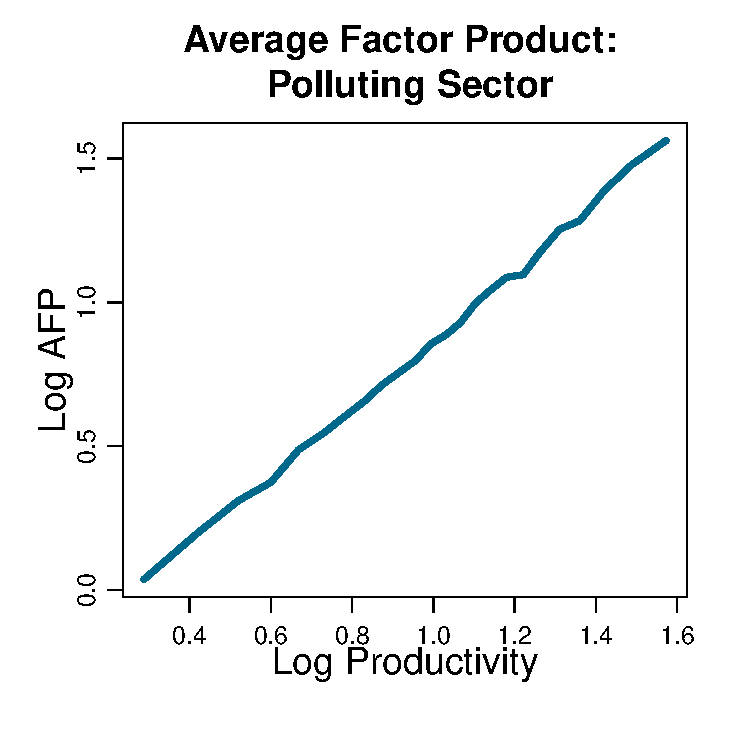
\includegraphics[width=0.40\textwidth]{./Figures/apf_pol_weight.pdf}
    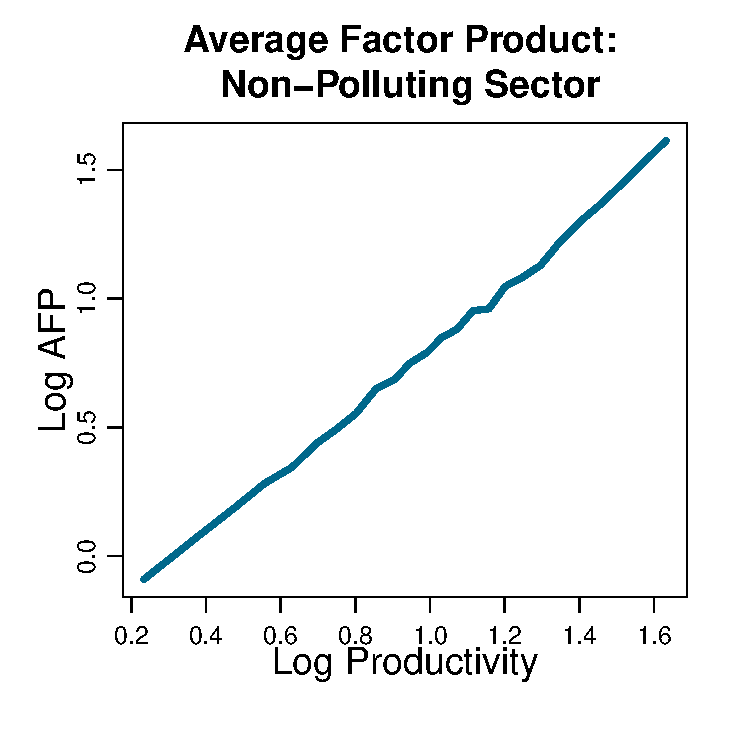
\includegraphics[width=0.40\textwidth]{./Figures/apf_npol_weight.pdf}
\end{center}
\end{figure}
\begin{itemize}
    \item
    Assume the correlated distortions are the same in both sectors:
    \begin{equation*}
        \tau_z = \max \left\{0,1-\phi_0 z^{\phi_1} \right\},
    \end{equation*}
    where $\tau_z$ is progressive when $\phi_1 < 0$.
\end{itemize}
\end{frame}

\begin{frame}[label=gedef]
\frametitle{Stationary Equilibrium}
\begin{itemize}
\itemsep=0.15in
    \item
    In the equilibrium, there are three thresholds:
    \begin{itemize}
        \itemsep=0.10in
        \item individuals choose to be manager iff $z > z_c (z_d)$ in each sector,
        \item firms in the polluting sector install clean technology iff $z > z_E$.
    \end{itemize}
    \item
    In the equilibrium,
    \begin{itemize}
        \itemsep=0.10in
        \item Household and firms optimize.
        \item Labor, capital and product markets clear.
        \item Aggregate emission:
        \begin{equation*}
            E = \mu\left[ \underbrace{\int_{z_d}^{{z}_E} e_0(y_z) dG(z)}_{\text{Dirty}} + \underbrace{\int_{{z}_E}^{\overline{z}} e_1(y_z) dG(z)}_{\text{Clean}} \right].
        \end{equation*}
    \end{itemize}
\end{itemize}
\hyperlink{firm_opt1}{\beamergotobutton{Optimization}}
\end{frame}

\begin{frame}[label=prop1]
\frametitle{Correlated Distortions and Technology Adoption}
\begin{figure}[htb]
\begin{center}
    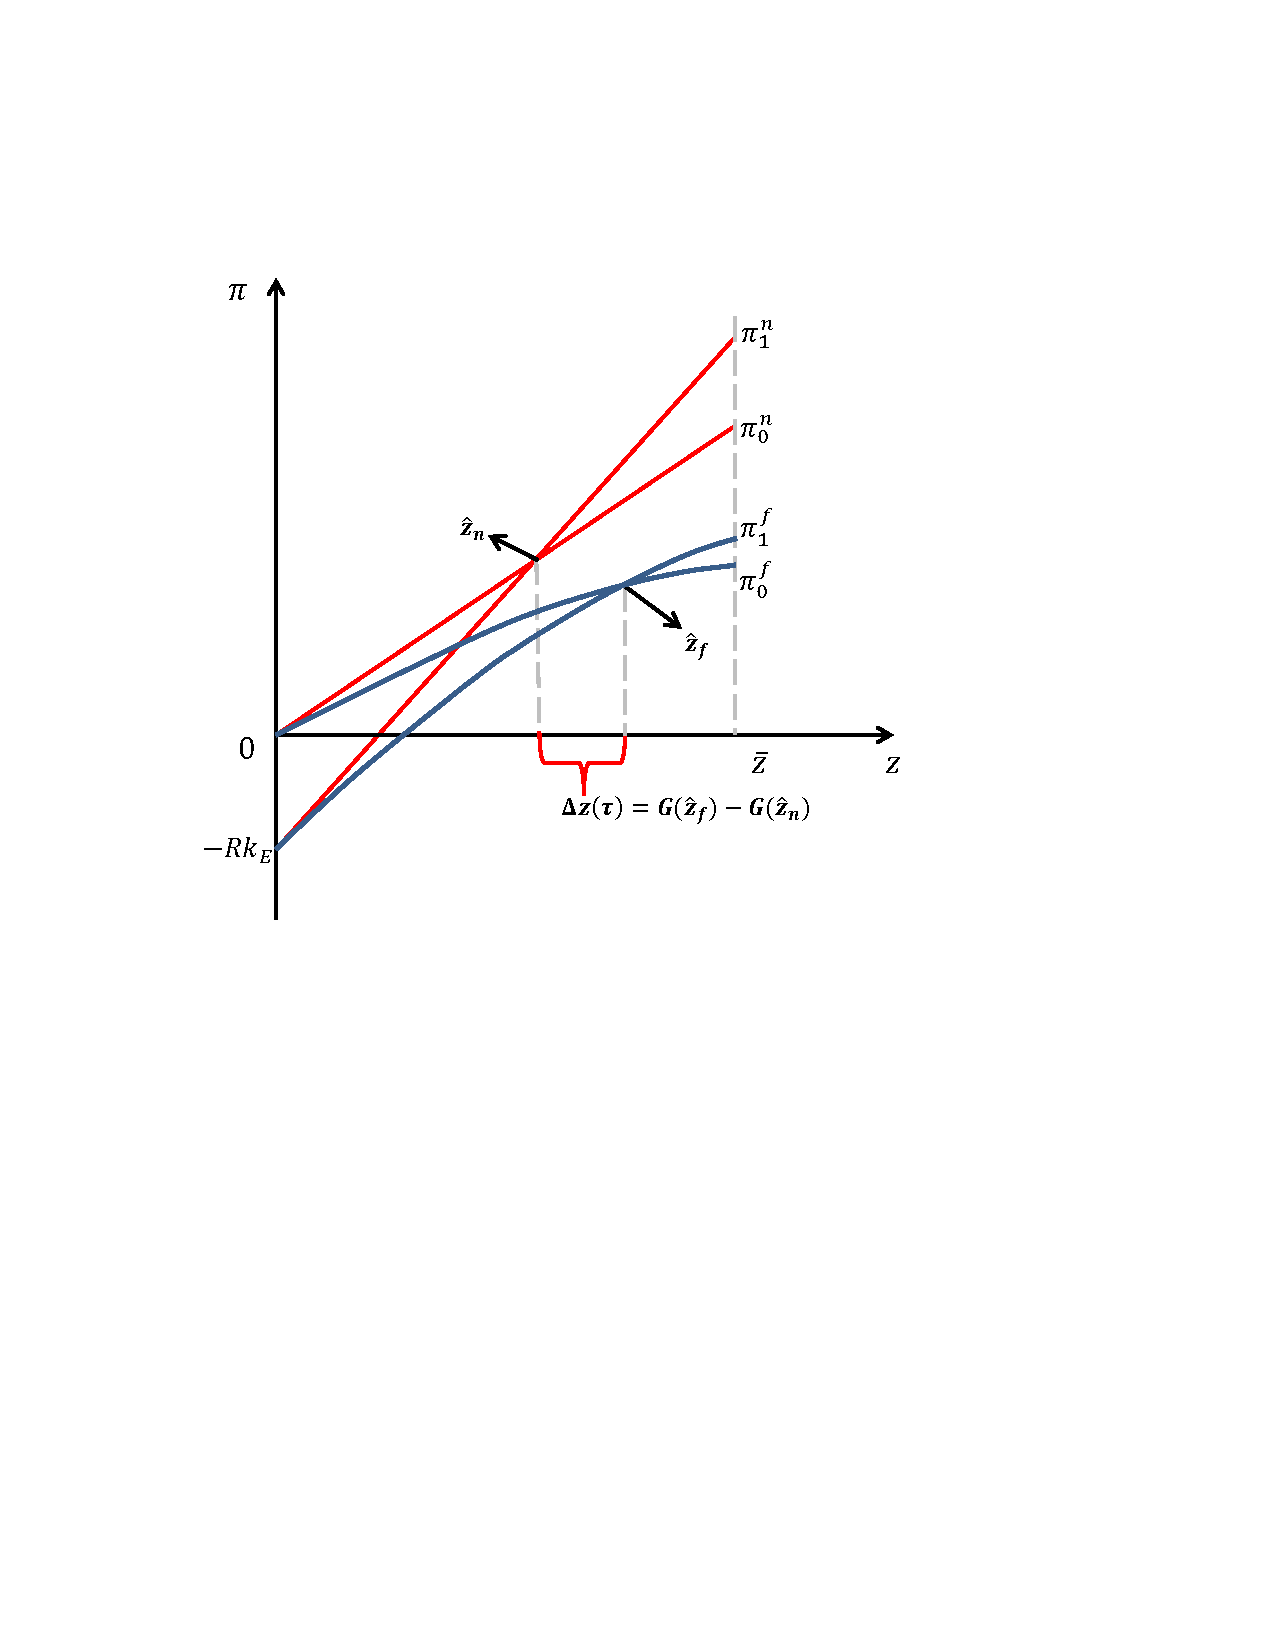
\includegraphics[width=0.60\textwidth]{./Figures/prod_tax_effect.pdf}
\end{center}
\end{figure}
\hyperlink{firm_opt2}{\beamergotobutton{Algebra}}
\end{frame}

\begin{frame}
\frametitle{Correlated Distortions and Aggregate Pollution}
\begin{itemize}
\itemsep=0.15in
    \item
    Consider a simplified one-sector model with no occupational and technology adoption choice.
    \item
    There exists a threshold
    \begin{equation*}
        \hat{\phi}_1 = \frac{\psi_1 (1-\gamma)}{1-\gamma(1+\psi_1)},
    \end{equation*}
    such that $E$ is decreasing in $|\phi_1|$ when $|\phi_1| < |\hat{\phi}_1|$.
    \item
    \btext{Intuition:}
    \begin{itemize}
        \item Technique effect dominates when the progressivity of the distortions is low.
        \item $|\hat{\phi}_1|$ is increasing in $|\psi_1|$.
    \end{itemize}
\end{itemize}
\end{frame}

\section{Quantitative Analysis}

\begin{frame}
\begin{center}
\LARGE{3. Quantitative Analysis}
\end{center}
\end{frame}

\begin{frame}
\frametitle{Calibration}
\framesubtitle{Calibration Strategy}
\begin{itemize}
\itemsep=0.15in
    \item
    \textit{\color{blue}Our Objective}: how firm size distribution affects aggregate pollution.
    \item
    Crucial to match the Chinese economy on:
    \begin{itemize}
        \item
        firm size distribution;
        \item
        relative distortions faced by large versus small firms;
        \item
        pollution intensity of differently sized firms.
    \end{itemize}
    \item
    $\tau_z$ and $G(z)$ jointly determine the firm size distribution.
    \item
    \textit{\color{blue}Identification}: Let $\theta_l = y/l$, then
    \begin{align*}
        \left(\frac{z_i}{z_j} \right)^{\phi_1} &= \frac{\theta_{l,j}}{\theta_{l,i}}, \\
        l^{1-\gamma} &= \Phi(1-\tau_z)z^{1-\gamma}.
    \end{align*}
\end{itemize}
\end{frame}

\begin{frame}
\frametitle{Calibration}
\framesubtitle{Parameterizations: Exogenously Calibrated}
\begin{table}[t]
\footnotesize
\centering
\begin{threeparttable}
\begin{tabular}{p{55pt}p{30pt}p{45pt}p{130pt}}
    \hline \hline
    Parameter   &                   & Value         & Target                                   \\
    \midrule
    Production  & $\delta$          & 0.1000        & Depreciation Rate                         \\
                & $\alpha$          & 0.5376        & Capital Share 0.5                         \\
                & $\mu$             & 0.20          & Fraction of firms in the polluting sector \\
    \midrule
    Treatment   & $\psi_0^{0}$      & $-$3.4144     & Physical Intensity-output Elasticity      \\
                & $\psi_1^{0}$      & $-$0.3636     & \\
                & $\psi_0^{1}$      & $-$4.3748     & Biological Intensity-output Elasticity    \\
                & $\psi_1^{1}$      & $-$0.3288     & \\
    \bottomrule
\end{tabular}
\end{threeparttable}
\end{table}
\end{frame}

\begin{frame}
\frametitle{Calibration}
\framesubtitle{Parameterizations: Endogenously Calibrated}
\begin{table}[t]
\footnotesize
\centering
\begin{threeparttable}
\begin{tabular}{p{55pt}p{30pt}p{45pt}p{135pt}}
    \hline \hline
    Parameter       &                   & Value         & Target                                   \\
    \midrule
    Treatment       & $k_E$             & 4.60          & Clean Firms: Fixed Cost/Output Ratio 2.5\%        \\
                    & $\xi$             & 0.23          & Clean Technology Adoption Rate 57\%            \\
    \midrule
    Preference      & $\beta$           & 0.8750        & Capital-output Ratio 1.65                 \\
    \midrule
    Distortions     & $\phi_0$          & 1.15          & Average Value Added Tax 13\%                   \\
                    & $\phi_1$          & $-$0.03       & $\theta_l$--$z$ Elasticity           \\
    \midrule
    Production      & $\gamma$          & 0.9300        & Size Distributions        \\
    \midrule
    Productivity    & $\mu$             & $-$2.4567     & Size Distributions        \\
                    & $\sigma$          & 4.0020        & \\
                    & $z'_{max}$        & 24855         & \\
                    & $g_{max}$         & 0.00048       & \\
    \bottomrule
\end{tabular}
\end{threeparttable}
\end{table}
\end{frame}

\begin{frame}[label=fitness]
\frametitle{Model Fit}
\begin{itemize}
    \item Size and Employment Distributions:
\end{itemize}
\begin{figure}[htb]
\begin{center}
    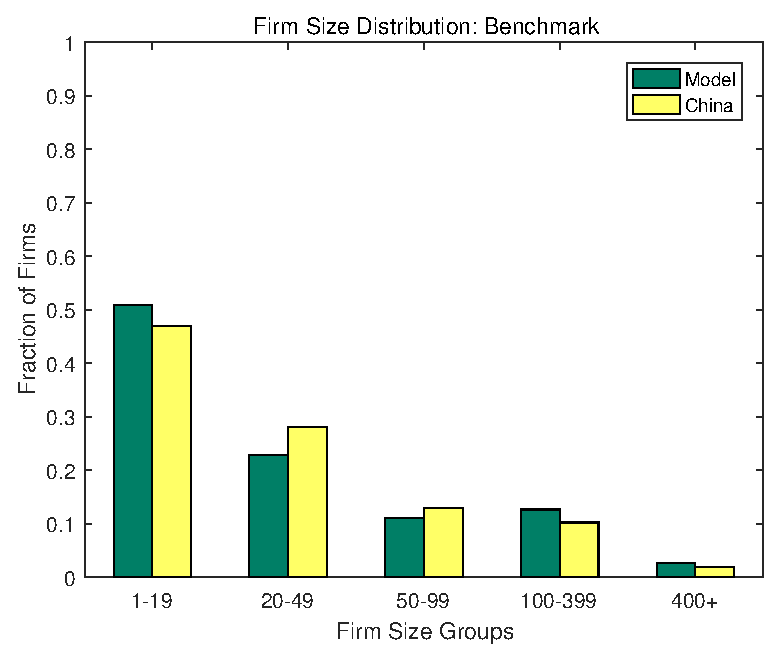
\includegraphics[width=0.45\textwidth]{./Figures/benchfit_fs.eps}
    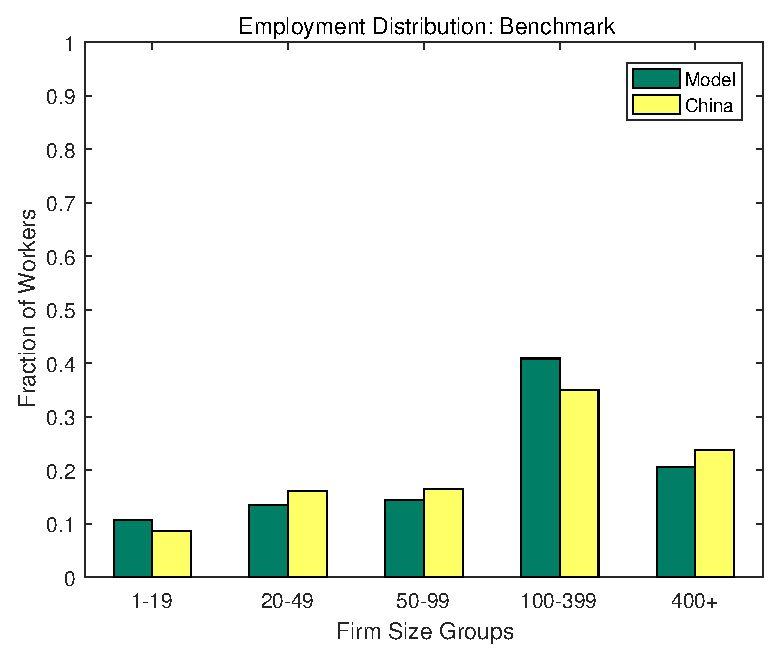
\includegraphics[width=0.45\textwidth]{./Figures/benchfit_es.eps}
\end{center}
\end{figure}
\end{frame}

\begin{frame}
\frametitle{Two Experiments}
\framesubtitle{Results}
\begin{itemize}
    \item
    Two Exercises:
    \begin{enumerate}[(i)]
        \item Removing all distortions.
        \item Increase regulation $\xi$ such that the fraction of firms using clean technology is the same 85\% as in (i).
    \end{enumerate}
    \item
    None of the exercises has large compositional effect, hence we focus on the polluting sector.
\end{itemize}
\begin{table}[t]
\footnotesize
\centering
\begin{threeparttable}
\begin{tabular}{p{85pt}p{45pt}p{45pt}p{35pt}}
    \hline \hline
    Statistic                       & Benchmark            & (i)                  & (ii)   \\
    \midrule
    Aggregate Output                & 100.0                & 131.2                & 99.0   \\
    Capital                         & 100.0                & 163.1                & 99.0   \\
    \midrule
    Number of Firms                 & 100.0                & 44.1                 & 89.9   \\
    Mean Size                       & 60                   & 139                  & 66     \\
    \midrule
    Aggregate Pollution             & 100.0                & 76.7                 & 85.8   \\
    Average Intensity               & 100.0                & 58.5                 & 86.7   \\
    Clean Share                     & 57.8                 & 85.6                 & 85.1   \\
    \bottomrule
\end{tabular}
\end{threeparttable}
\end{table}
\end{frame}

\begin{frame}
\frametitle{Mechanism}
\framesubtitle{No Distortions}
\begin{figure}[htb]
\begin{center}
  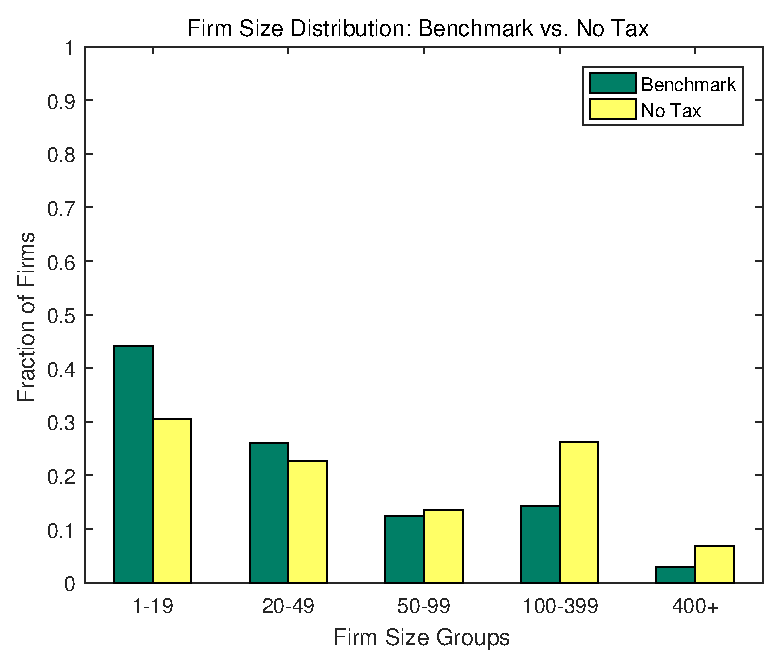
\includegraphics[width=0.45\textwidth]{./Figures/bench_notax_fs.eps}
  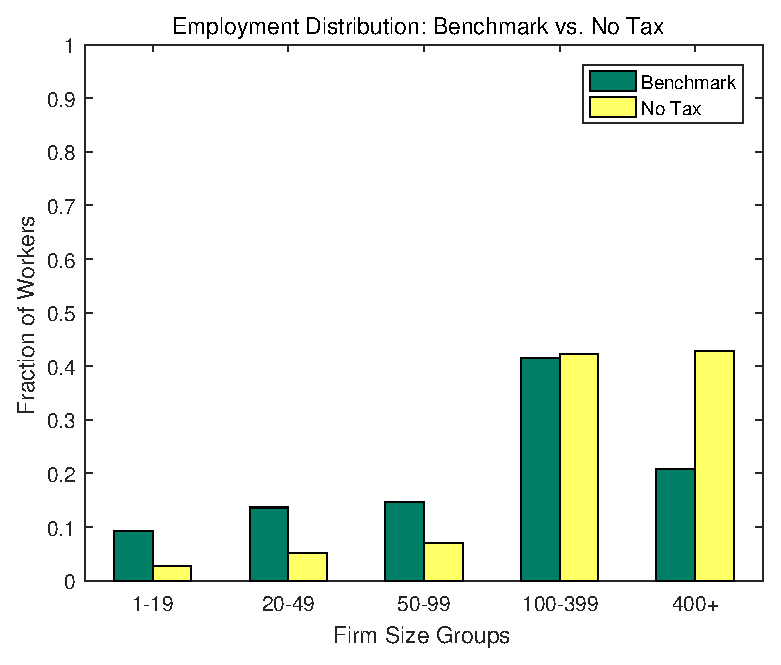
\includegraphics[width=0.45\textwidth]{./Figures/bench_notax_es.eps}
\end{center}
\end{figure}
\end{frame}

\begin{frame}
\frametitle{Mechanism}
\framesubtitle{Stronger Regulations}
\begin{figure}[htb]
\begin{center}
  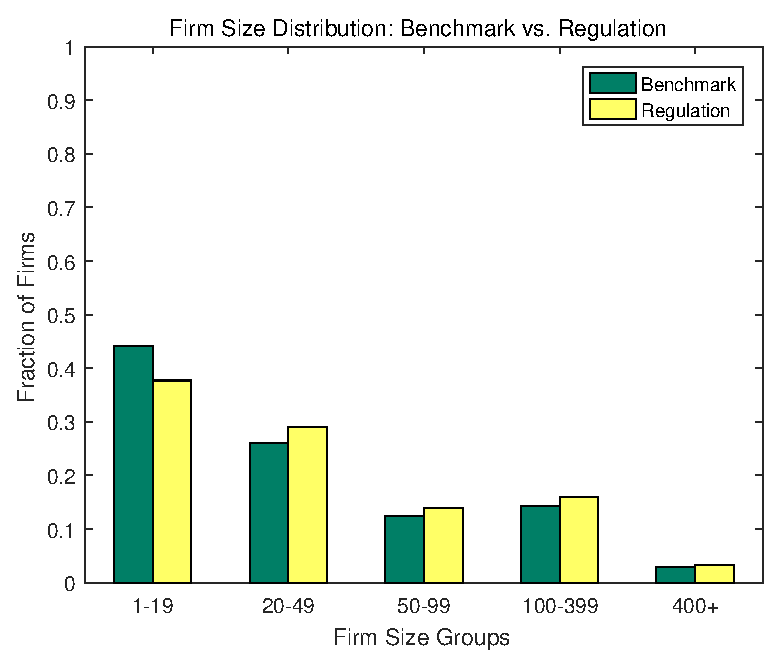
\includegraphics[width=0.45\textwidth]{./Figures/bench_reg_fs.eps}
  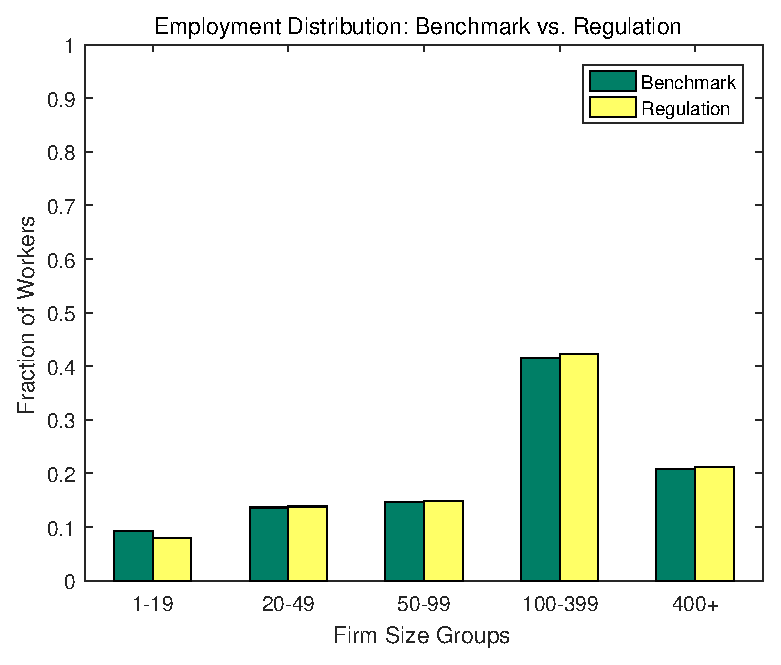
\includegraphics[width=0.45\textwidth]{./Figures/bench_reg_es.eps}
\end{center}
\end{figure}
\end{frame}

\begin{frame}[label=geresults]
%\small
\frametitle{Mechanism}
\framesubtitle{Misallocation}
\begin{itemize}
\itemsep=0.15in
    \item
    {\color{black}Extensive} and {{\color{black}Intensive}} Margin:
    \begin{itemize}
    \item {\color{black}Extensive margin}: selection of more productive firms.
    \item {\color{black}Intensive margin}: production distribution among active firms.
    \end{itemize}
    \begin{table}[t]
    \footnotesize
    \centering
    \begin{threeparttable}
    \begin{tabular}{p{45pt}p{25pt}p{25pt}p{25pt}p{25pt}p{25pt}}
        \hline \hline
        Economy     & $\text{QU}_1$ & $\text{QU}_2$ & $\text{QU}_3$ & $\text{QU}_4$ & $\text{QU}_5$ \\
        \midrule
        Benchmark   & 2.79          & 4.26          & 7.45          & 16.81         & 68.70 \\
        Case (i)    & 1.53          & 2.89          & 6.46          & 18.25         & 70.87 \\
        Case (ii)   & 3.02          & 4.63          & 8.01          & 17.79         & 66.55 \\
        \bottomrule
    \end{tabular}
    \end{threeparttable}
    \end{table}
    \item
    Regulations {\color{red}worsen} resource allocation on the intensive margin by amplifying the effects of distortions.
    \item
    Core mechanics:
    \begin{itemize}
        \item
        General equilibrium feedback through wages.
        \item
        The interaction between selection and correlated distortions.
    \end{itemize}
\end{itemize}
\hyperlink{peresults}{\beamergotobutton{Monopolistic Competition}}
\end{frame}

\begin{frame}[label=sizedepen]
\frametitle{Mechanism}
\framesubtitle{The Progressiveness in Distortions}
\begin{itemize}
    \item Experiment (i') imposes a uniform distortion to all the firms that collects the same amount of tax revenue.
\end{itemize}
\begin{table}[t]
\footnotesize
\centering
\begin{threeparttable}
\begin{tabular}{p{85pt}p{45pt}p{45pt}p{25pt}}
    \hline \hline
    Statistic                & Benchmark            & (i')            & (i)   \\
    \midrule
    Aggregate Output         & 100.0                & 108.2           & 131.2  \\
    Capital                  & 100.0                & 110.9           & 163.1  \\
    \midrule
    Number of Firms          & 100.0                & 44.1            & 44.1   \\
    Mean Size                & 60                   & 139             & 139    \\
    \midrule
    Aggregate Pollution      & 100.0                & 70.0            & 76.7   \\
    Average Intensity        & 100.0                & 64.8            & 58.5   \\
    Clean Share              & 57.4                 & 73.3            & 85.6   \\
    \bottomrule
\end{tabular}
\end{threeparttable}
\end{table}
\begin{itemize}
    \item
    The progressiveness of the distortions is particularly damaging to the environment.
\end{itemize}
\end{frame}

\begin{frame}
\frametitle{Compositional Effect}
\framesubtitle{Setting}
\begin{itemize}
    \item
    Consider when the products from the two sectors have a constant elasticity of substitution $\rho$:
    \begin{equation*}
        Y = \left[\varphi(Y_d)^{\frac{\rho-1}{\rho}} + (1-\varphi)(Y_c)^{\frac{\rho-1}{\rho}} \right]^{\frac{\rho}{\rho-1}}.
    \end{equation*}
    \item
    The price of the final good $Y$ is normalized to one:
    \begin{equation*}
        \left[ \varphi^{\rho} p_d^{1-\rho} + (1-\varphi)^{\rho} p_c^{1-\rho} \right]^{\frac{1}{\rho-1}} = 1.
    \end{equation*}
    \item
    Two Exercises:
    \begin{enumerate}[(i)]
        \item Removing all distortions.
        \item Removing only the distortions in the polluting sector.
    \end{enumerate}
\end{itemize}
\end{frame}

\begin{frame}
\frametitle{Compositional Effect}
\framesubtitle{Results}
\begin{table}[t]
\footnotesize
\centering
\begin{threeparttable}
\begin{tabular}{lccccccc}
    \hline \hline
                         & \multicolumn{3}{c}{Polluting}    & & \multicolumn{3}{c}{Non-polluting} \\
    \cmidrule{2-4} \cmidrule{6-8}
    Statistics           & Benchmark & (i)      & (ii)      & & Benchmark     & (i)    & (ii) \\
    \midrule
    Physical Output      & 100.00    & 129.64   & 134.63    & & 100.00        & 129.90 &  98.03 \\
    Price                & 100.00    & 99.97    & 85.00     & & 100.00        & 100.00 & 102.34 \\
    Revenue              & 100.00    & 129.60   & 114.42    & & 100.00        & 129.90 & 100.32 \\
    \midrule
    \# of Firms          & 100.00    & 42.63    & 46.44     & & 100.00        & 41.88  &  95.38 \\
    Mean Size            & 64.31     & 152.21   & 176.17    & & 51.16         & 123.50 &  49.38 \\
    \midrule
    Pollution            & 100       & 74.69    & 80.05     \\
    Intensity            & 100       & 57.81    & 59.47     \\
    Clean Share          & 56.18     & 83.80    & 73.10     \\
    \bottomrule
\end{tabular}
\end{threeparttable}
\end{table}
\end{frame}

\section{Conclusion}
\begin{frame}
\frametitle{Conclusions}
\begin{itemize}
\itemsep=0.15in
    \item
    This paper proposes a new explanation for the industrial pollution problem in China:
    \begin{itemize}
        \item
        a negative relationship between firm size and the pollution intensity;
        \item
        expansion of productive firms is limited by distortions.
    \end{itemize}
    \item
    We build a model consistent with the empirical regularities.
    \item
    Quantitative results show that distortions reduce output by 30\% and increase pollution by 20\%.
    \item
    Regulations improves resource allocation on the extensive margin, but worsens the intensive margin by amplifying distortions.
\end{itemize}
\end{frame}

%\begin{frame}
%\frametitle{Future Research}
%\begin{itemize}
%\itemsep=0.15in
%    \item
%    Agricultural Sector:
%    \begin{itemize}
%        \item
%        Our PNAS paper: Land and migration policies on fertilizer intensity.
%        \item
%        What drives the difference in cropping practice of small versus large farmers?
%        \item
%        What are the structural transformation implications of land consolidation (Hornbeck, 2012, 2014; Bustos et al., 2016; Henderson et al. 2018)?
%    \end{itemize}
%    \item
%    Spatial Distribution of Pollution:
%    \begin{itemize}
%        \item
%        Different forces of economic agglomeration (Combes et al., 2012; Gaubert, 2018).
%        \item
%        Preliminary analysis of the data shows that economic-advanced regions have lower pollution intensity.
%        \item
%        What are the environmental consequences of regional development policies (Kline and Moretti, 2014)?
%    \end{itemize}
%    \item
%    Trade and Structural Change:
%    \begin{itemize}
%        \item
%        The theory of mass consumption (Matsuyama, 2002; Faber and Fally, 2017).
%        \item
%        Economic Density (Holmes, 2011; Lagakos, 2016).
%    \end{itemize}
%\end{itemize}
%\end{frame}

\begin{frame}
\begin{center}
\LARGE{Thank You!}
\end{center}
\end{frame}

\section{Appendix}

\begin{frame}
\begin{center}
\LARGE{Appendix}
\end{center}
\end{frame}

\begin{frame}[label=coddef]
\small
\frametitle{Chemical Oxygen Demand Definition}
\begin{itemize}
\itemsep=0.15in
    \item
    In environmental chemistry, the chemical oxygen demand (COD) test is commonly used to {\color{black}indirectly measure the amount of organic compounds in water}. Most applications of COD determine the amount of organic pollutants found in surface water (e.g. lakes and rivers) or waste water, making COD a useful measure of water quality. It is expressed in milligrams per liter (mg/L) also referred to as ppm (parts per million), which indicates the mass of oxygen consumed per liter of solution.
    \item
    COD is an indirect measure that indicates the presence of contaminants that will eventually cause oxygen loss.
\end{itemize}
\hyperlink{datasource}{\beamergotobutton{Data Source}}
\end{frame}

\begin{frame}[label=pollutants]
\frametitle{Major Pollutant Discharge}
\begin{table}[t]
\footnotesize
\centering
\begin{threeparttable}
\begin{tabular}{lcccccccccc}
    \hline \hline
        & Waste & COD  & Petro & $\text{NH}_4^+$ & BOD  & CN   & $\text{Cr}^{6+}$ & Phenol & As   & Cr   \\
    \midrule
    Key & 76.2  & 73.2 & 31.4  & 25.2            & 17.5 & 4.90 & 4.86             & 2.42   & 2.27 & 2.01 \\
    Reg & 35.2  & 28.3 & 7.91  & 6.49            & 2.56 & 0.13 & N/A              & 0.04   & 0.07 & N/A  \\
    \bottomrule
\end{tabular}
\begin{tablenotes}
     \footnotesize{\item[$\dagger$]
     Data Source: National General Survey of Pollution Sources. \\
     Acronyms: \\
     {\color{purpledef}Waste}: Wastewater; {\color{purpledef}COD}: Chemical Oxygen Demand; {\color{purpledef}Petro}: Petrochemicals; {\color{purpledef}$\text{NH}_4^+$}: Ammonian \\
     {\color{purpledef}BOD}: Biochemical Oxygen Demand; {\color{purpledef}CN}: Cyanidium; {\color{purpledef}$\text{Cr}^{6+}$}: Hexavalent Chromium \\
     {\color{purpledef}Phenol}: Volatile Phenols; {\color{purpledef}As}: Arsenium; {\color{purpledef}Cr}: Chromium.}
\end{tablenotes}
\label{tab:nfirmPollutant}
\end{threeparttable}
\end{table}
\hyperlink{datasource}{\beamergotobutton{Data Sources}}
\end{frame}

\begin{frame}[label=codscatter]
\frametitle{Firm Size and Pollution Intensity}
\makebox[\linewidth]{%
  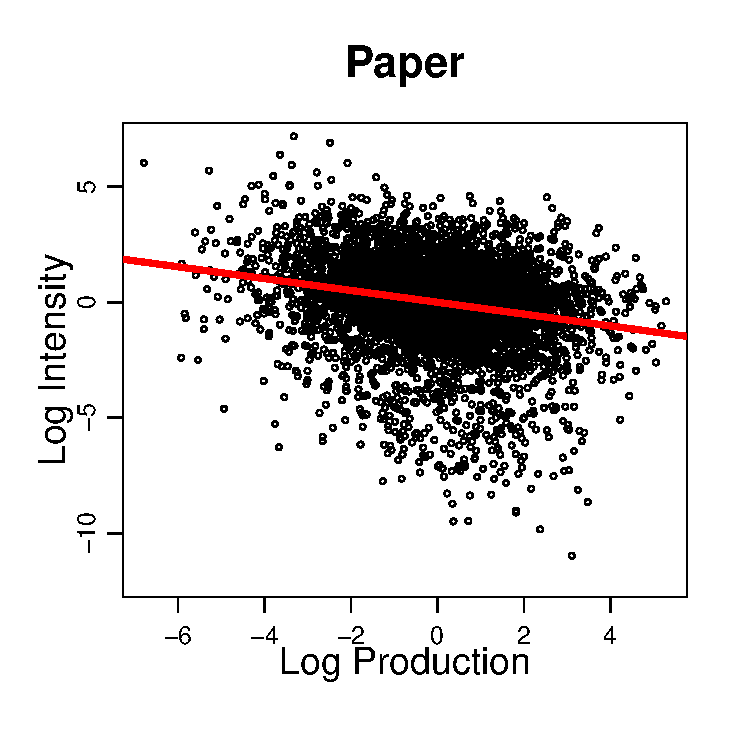
\includegraphics[width=0.3\textwidth]{./Figures/paper_ez.pdf}%
  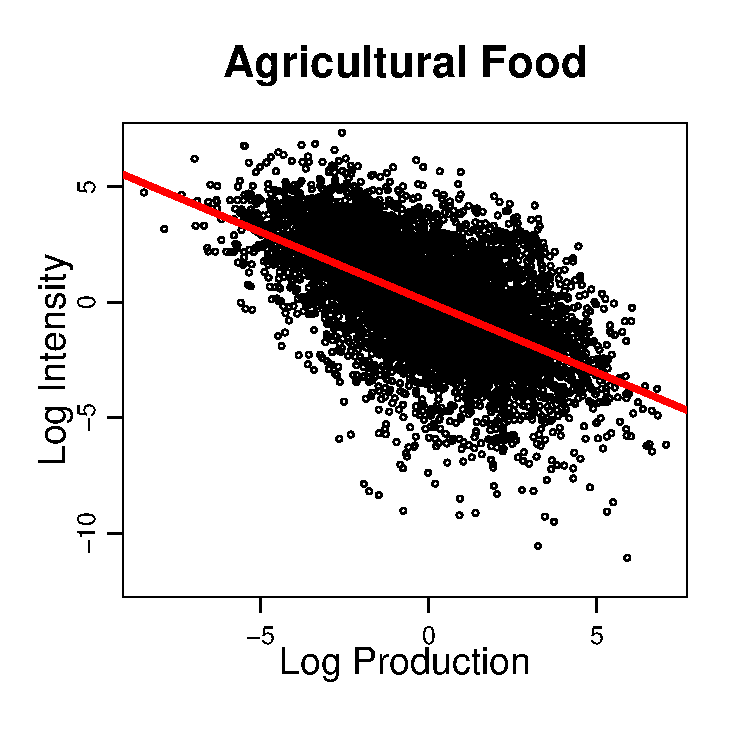
\includegraphics[width=0.3\textwidth]{./Figures/agri_ez.pdf}
  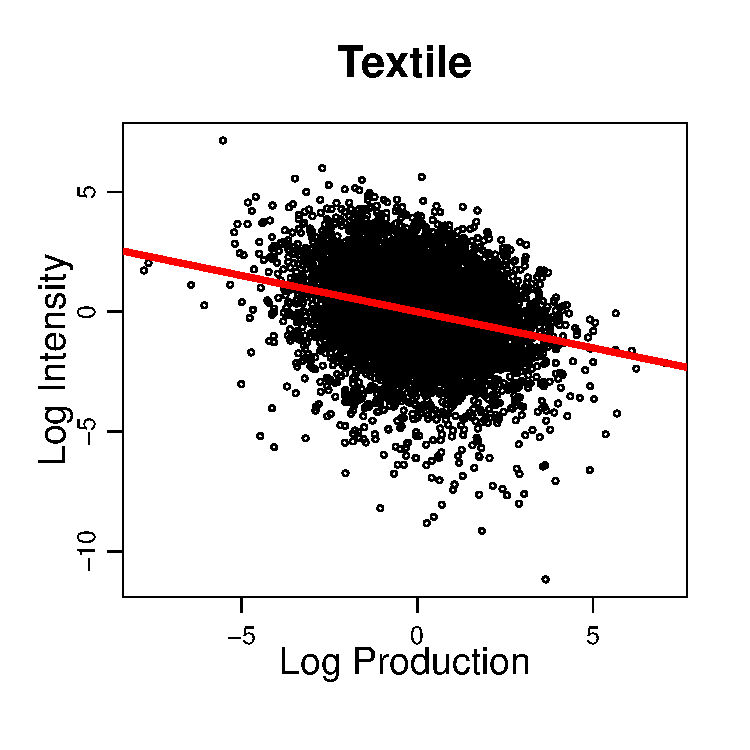
\includegraphics[width=0.3\textwidth]{./Figures/text_ez.pdf}}
\\
\makebox[\linewidth]{%
  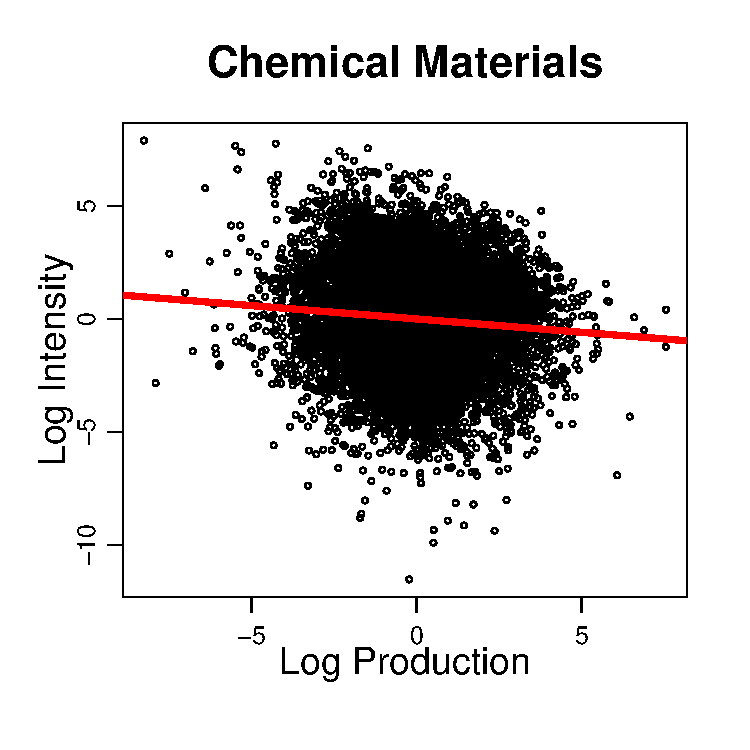
\includegraphics[width=0.3\textwidth]{./Figures/chem_ez.pdf}
  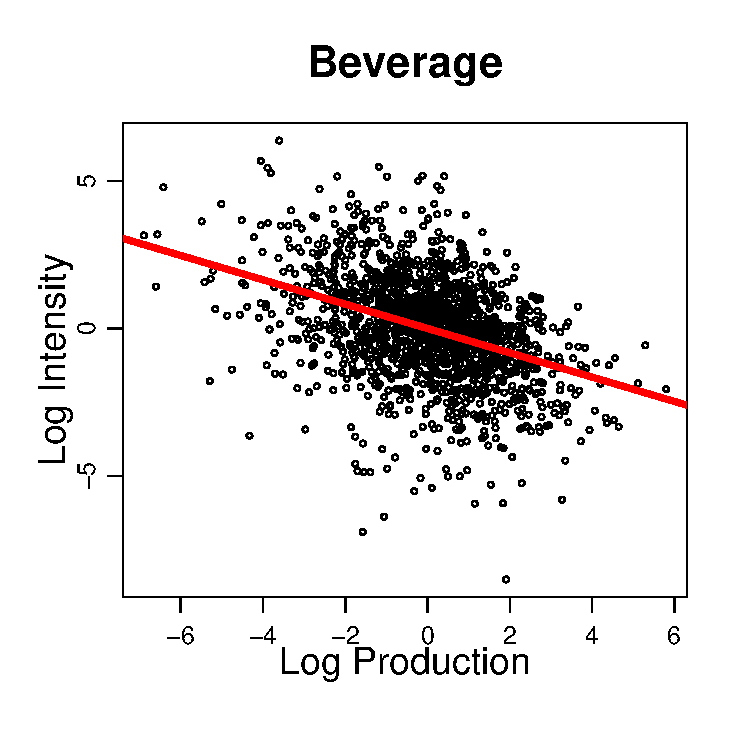
\includegraphics[width=0.3\textwidth]{./Figures/bever_ez.pdf}
  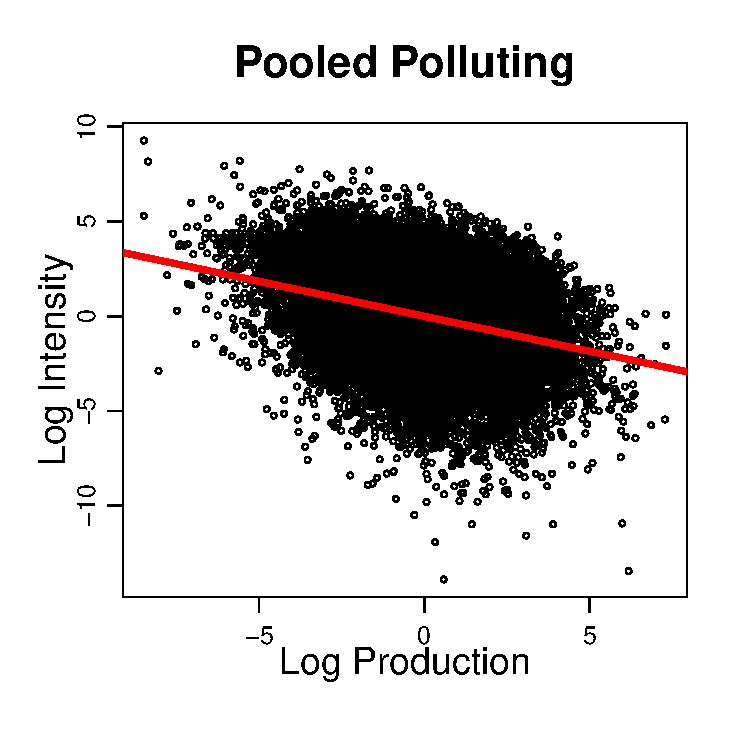
\includegraphics[width=0.3\textwidth]{./Figures/pooled_intensity_size.pdf}}
\end{frame}

\begin{frame}[label=treatment2]
\small
\frametitle{Treatment Technologies}
\framesubtitle{Efficiency of Technologies}
\begin{itemize}
\itemsep=0.15in
    \item
    Examples of the treatment technologies:
    \begin{itemize}
    \item {\color{black}Physical}: Filtering, Centrifuging, Precipitation Separation, etc.
    \item {\color{black}Chemical}: Oxidation-reduction, neutralization, etc.
    \item {\color{black}Biological}: Aerobic Biological Treatment, Activated Sludge Process, etc.
    \end{itemize}
    \item
    In the U.S. wastewater treatment system,
    \begin{itemize}
        \item
        Physical technology: preliminary and primary treatments.
        \item
        Chemical and biological technologies: secondary and tertiary treatments.
    \end{itemize}
\end{itemize}
\hyperlink{treatment1}{\beamergotobutton{Treatment Technology}}
\end{frame}

\begin{frame}[label=treattech2]
\small
\frametitle{Treatment Technologies}
\framesubtitle{Costs, Capacity and Production Scale}
\makebox[\linewidth]{
    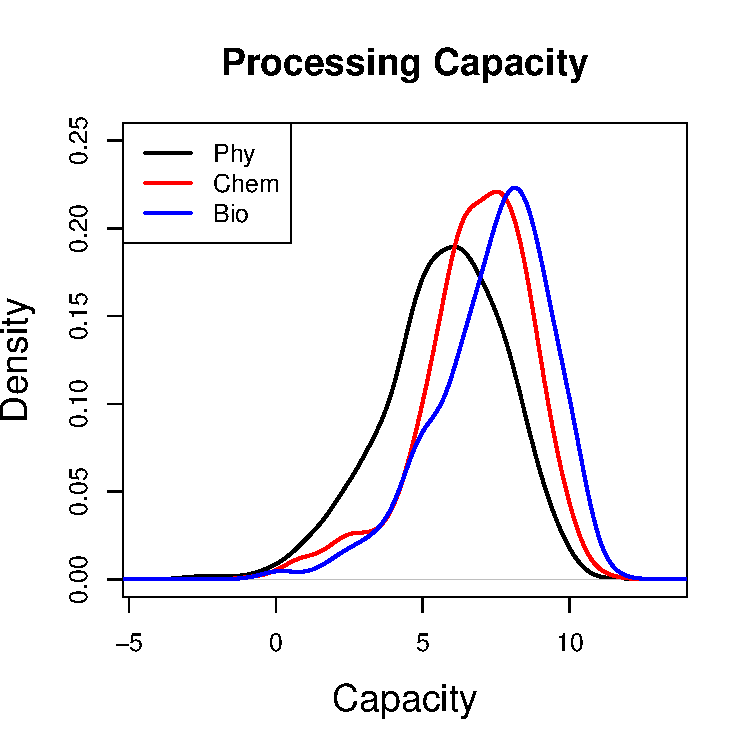
\includegraphics[width=0.33\textwidth]{./Figures/abate_cap.pdf}
    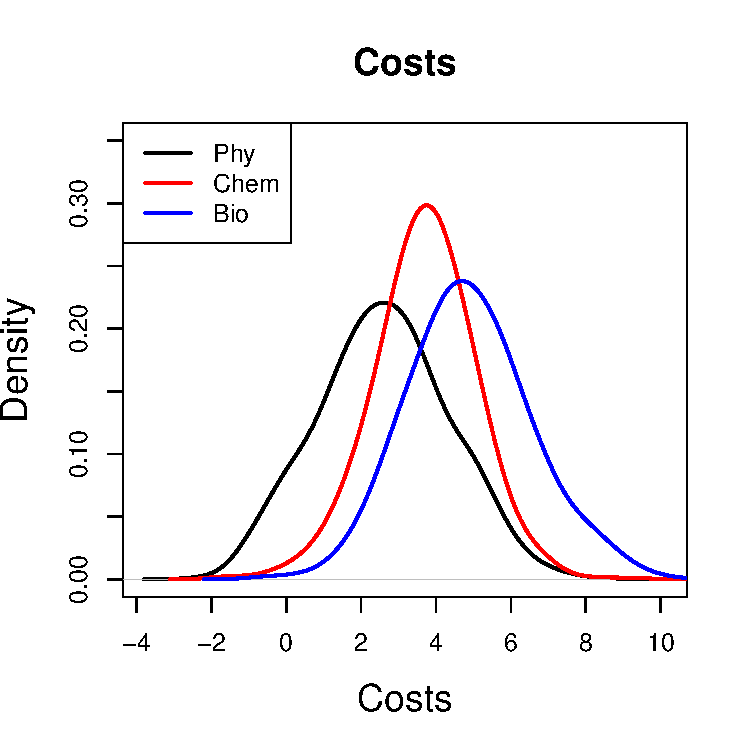
\includegraphics[width=0.33\textwidth]{./Figures/abate_inv.pdf}}
\\
\makebox[\linewidth]{
    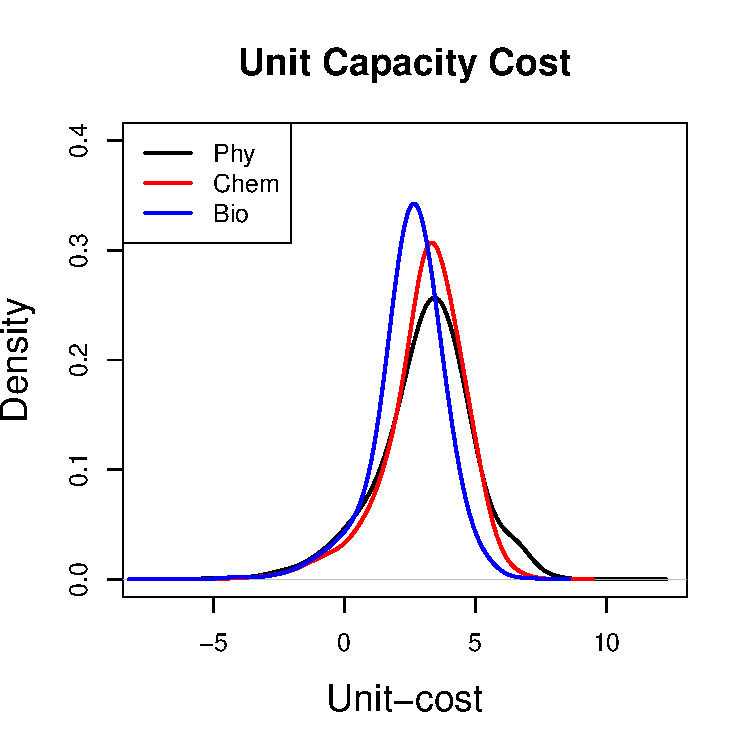
\includegraphics[width=0.33\textwidth]{./Figures/abate_unit.pdf}
    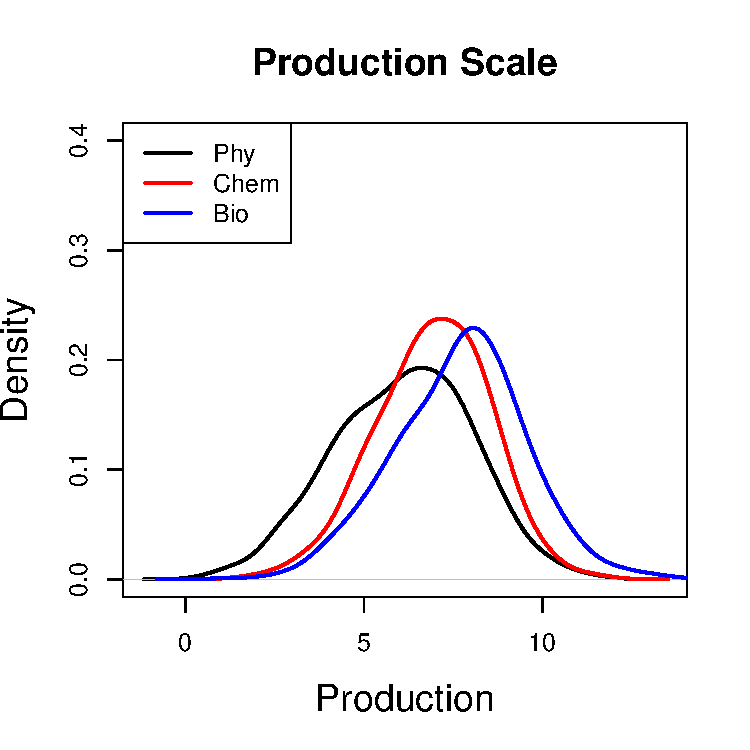
\includegraphics[width=0.33\textwidth]{./Figures/abate_prod.pdf}}
\hyperlink{treatment1}{\beamergotobutton{Treatment Technology}}
\end{frame}

\begin{frame}[label=esdist]
\frametitle{Firm Size Distribution}
\framesubtitle{By Industry}
\makebox[\linewidth]{%
  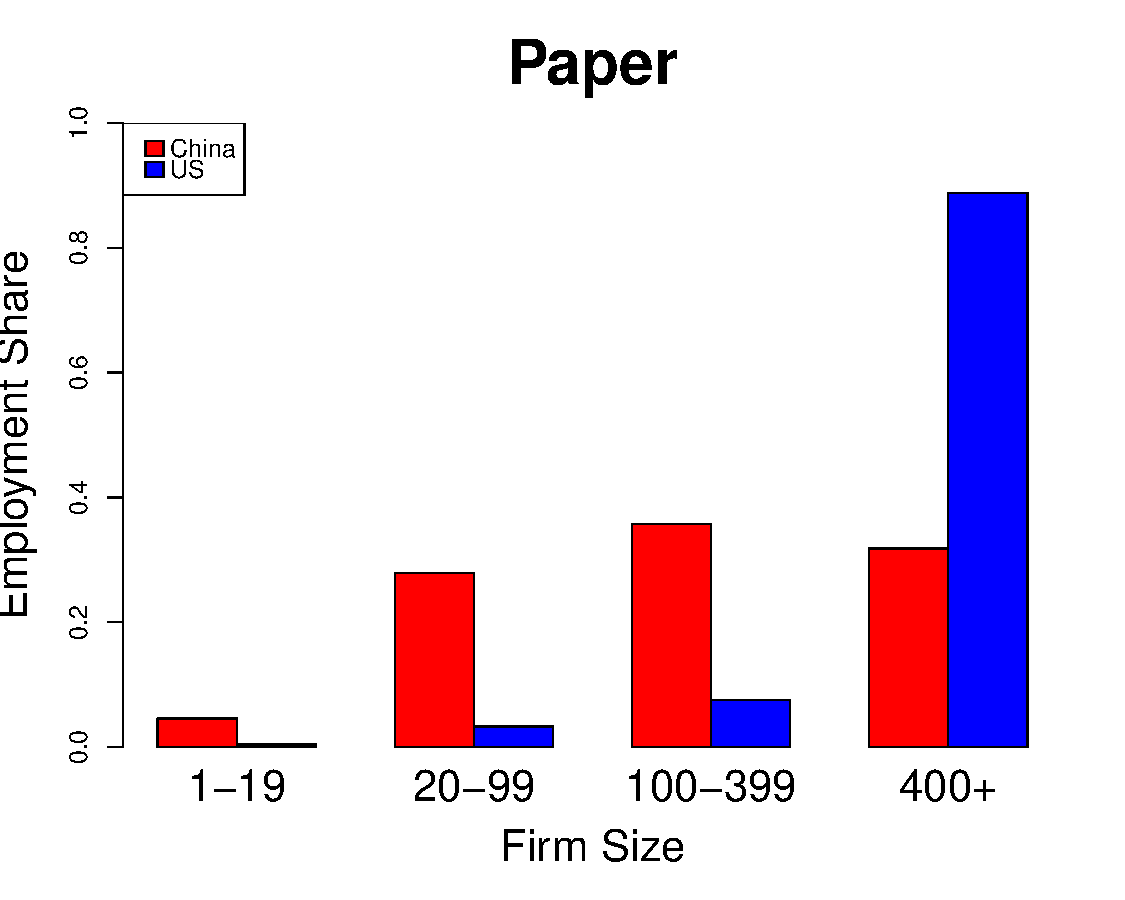
\includegraphics[width=0.3\paperwidth,height=0.35\paperheight]{D:/PaperDrafts/Pollution/R_Implementation/paperES_R.pdf}%
  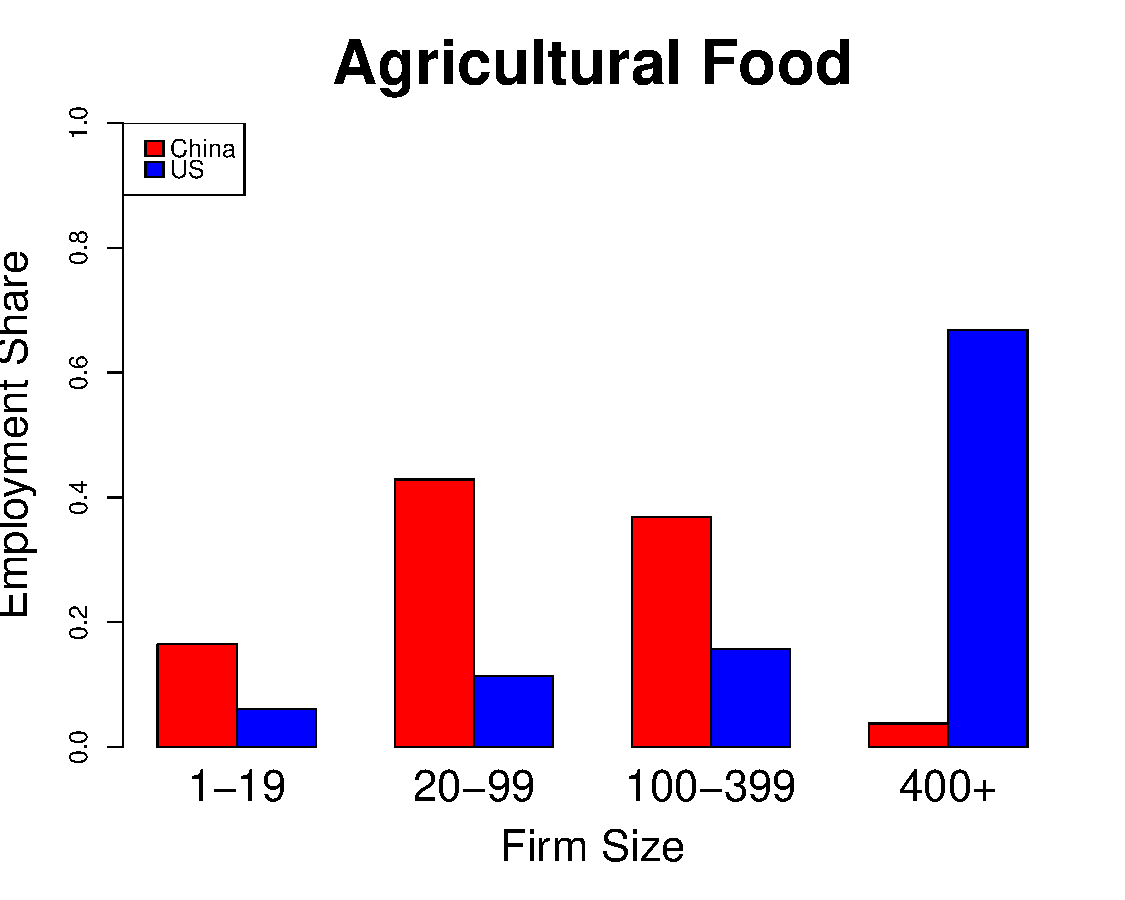
\includegraphics[width=0.3\paperwidth,height=0.35\paperheight]{D:/PaperDrafts/Pollution/R_Implementation/agriES_R.pdf}
  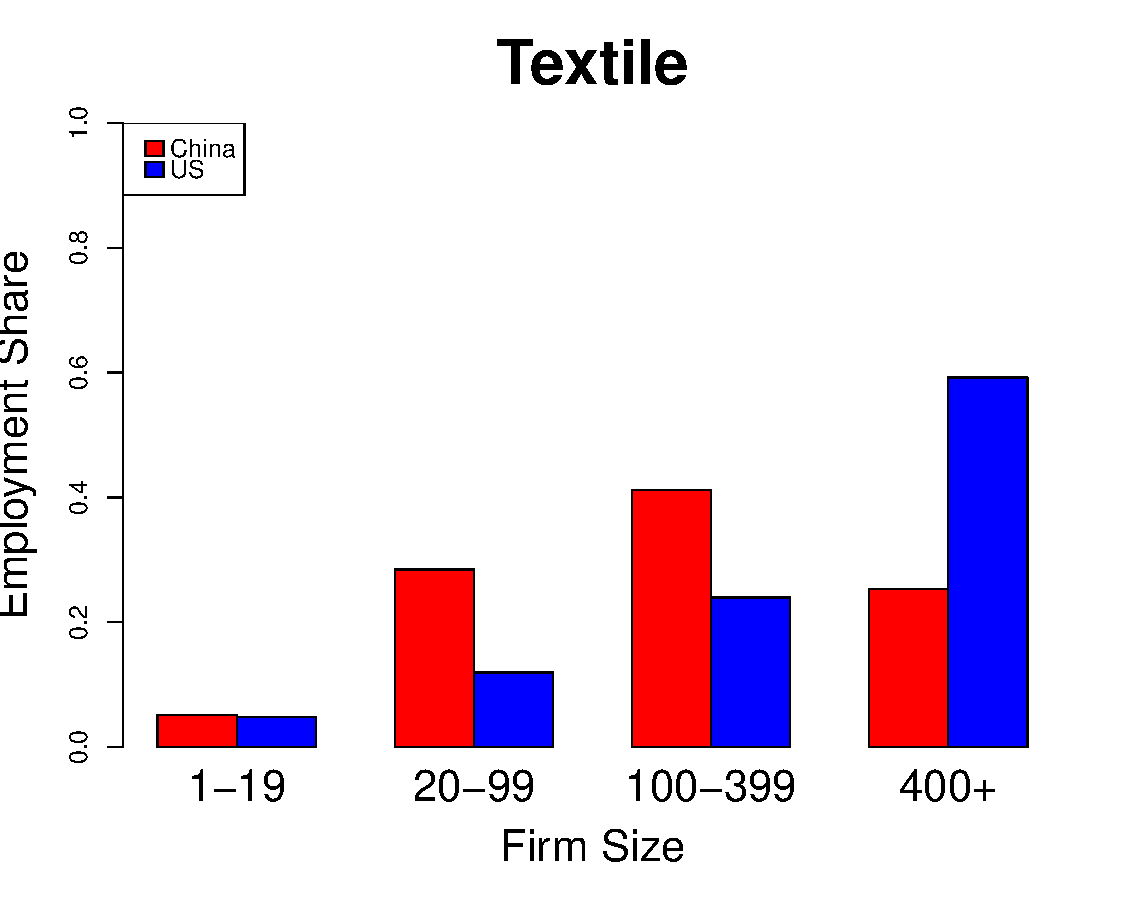
\includegraphics[width=0.3\paperwidth,height=0.35\paperheight]{D:/PaperDrafts/Pollution/R_Implementation/textileES_R.pdf}}
\\
\makebox[\linewidth]{%
  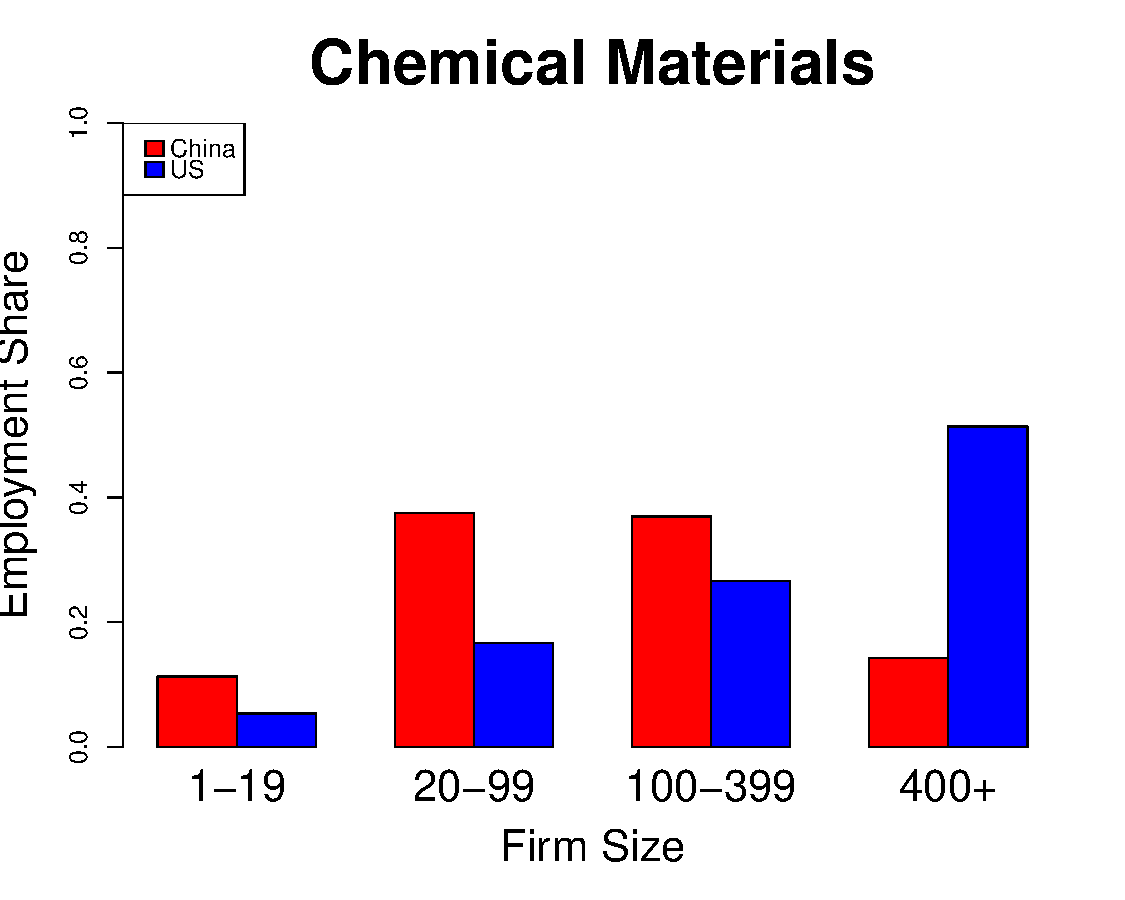
\includegraphics[width=0.3\paperwidth,height=0.35\paperheight]{D:/PaperDrafts/Pollution/R_Implementation/chemmatES_R.pdf}
  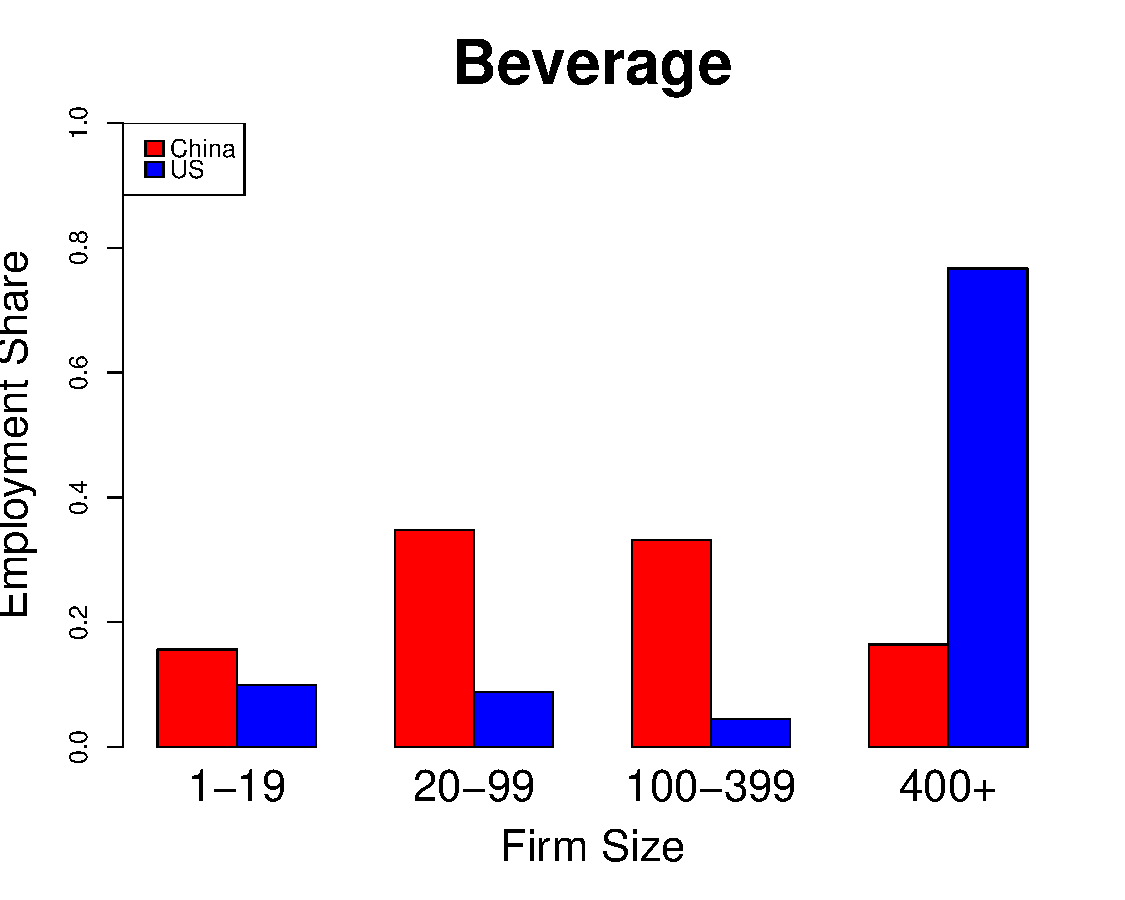
\includegraphics[width=0.3\paperwidth,height=0.35\paperheight]{D:/PaperDrafts/Pollution/R_Implementation/beverES_R.pdf}
  \includegraphics[width=0.3\paperwidth,height=0.35\paperheight]{D:/PaperDrafts/Pollution/R_Implementation/poolES_R.pdf}}
\hyperlink{esdistall}{\beamergotobutton{Polluting and All Manufacturing}}
\end{frame}

\begin{frame}[label=accountingrbst]
\small
\frametitle{Robustness of the Accounting Exercise}
\begin{itemize}
    \item
    We need to estimate the employment--production relationship of Chinese firms because
    \begin{itemize}
    \item the U.S data contain only information on number of employees;
    \item the pollution census has information on production, but {\color{black}not} on number of employees.
    \end{itemize}
    \item
    China National Economic Census data are used.
    \item
    Results:
    \begin{table}[t]
    \footnotesize
    \centering
    \begin{threeparttable}
    %\caption{Size Distribution on Pollution}
    \begin{tabular}{lccccccc}
        \hline \hline
        Method             & Paper  & Agri   & Tex    & Chem    & Bever        & Pooled & Reduc  \\
        \midrule
        Non-parametric      & 39.8\% & 60.7\% & 81.6\% & 102.5\% & 103.7\%      & 63.5\% & 28.2\% \\
        Piecewise-linear    & 34.8\% & 69.4\% & 93.5\% & 180.1\% & N/A          & 75.4\% & 19.0\% \\
        Parametric          & 43.5\% & 61.1\% & 97.5\% & 101.2\% & 89.0\%       & 67.0\% & 25.5\% \\
        \bottomrule
    \end{tabular}
    \end{threeparttable}
    \end{table}
\end{itemize}
\hyperlink{accounting}{\beamergotobutton{Accounting Exercise}}
\end{frame}

\begin{frame}[label=firm_opt1]
\frametitle{Firm's Optimization}
\framesubtitle{Setting}
\begin{itemize}
    \item
    Non-polluting sector:
    \begin{equation*}
        \pi^c(z) = \max_{k,l}\left\{(1-\tau_z)z^{1-\gamma}(k^{\alpha}l^{1-\alpha})^{\gamma} - Wl - Rk \right\}.
    \end{equation*}
    \item
    Polluting sector:
    \begin{itemize}
        \item
        Technology Adoption:
        \begin{equation*}
            \pi^d(z) = \max_{i \in \{0,1\}} \left\{ \pi^d_0(z), \pi^d_1(z) \right\}.
        \end{equation*}
        \item
        Profits when using dirty technology
        \begin{equation*}
            \pi^d_0(z) = \max_{k,l} \left\{ (1-\xi )\left[ \left( 1-\tau_z \right) z^{1-\gamma} (k^{\alpha} l^{1-\alpha})^{\gamma} - Wl - Rk \right] \right\}.
        \end{equation*}
        \item
        Profits when using clean technology
        \begin{equation*}
            \pi^d_1(z) = \max_{k,l} \left\{\left( 1-\tau_z \right) z^{1-\gamma} (k^{\alpha} l^{1-\alpha})^{\gamma} - Wl - R(k+k_E) \right\}.
        \end{equation*}
    \end{itemize}
\end{itemize}
\hyperlink{gedef}{\beamergotobutton{Equilibrium}}
\end{frame}

\begin{frame}[label=firm_opt2]
\frametitle{Firm's Optimization}
\framesubtitle{Technology Adoption Decision}
\begin{itemize}
\itemsep=0.15in
    \item
    Difference in potential profits using different technologies:
    \begin{equation*}
        \pi_1^d(z) - \pi_0^d(z) = \frac{\xi (1-\gamma)}{(1-\alpha)\gamma} W l^d(z) - Rk_E.
    \end{equation*}
    \item
    There exists a threshold $z^E$ where firms switch technology.
    \begin{itemize}
    \itemsep=0.10in
        \item
        $z_E$ increases with $\xi$ and decreases with $k_E$.
        \item
        $z_E$ increases with $\tau_z$.
    \end{itemize}
\end{itemize}
\hyperlink{prop1}{\beamergotobutton{Graphical}}
\end{frame}

\begin{frame}[label=fitness1]
\frametitle{Model Fit Benchmark Full Groups}
\makebox[\linewidth]{
    \includegraphics[width=0.45\paperwidth,height=0.45\paperheight]{D:/PaperDrafts/Pollution/PrelimResults/sizedist_china_full.eps}
    \includegraphics[width=0.45\paperwidth,height=0.45\paperheight]{D:/PaperDrafts/Pollution/PrelimResults/eshare_china_full.eps}}
\hyperlink{fitness}{\beamergotobutton{Model Fit}}
\end{frame}

\begin{frame}[label=peresults]
\frametitle{Monopolistic Competition}
\framesubtitle{Setting}
\begin{itemize}
\itemsep=0.15in
    \item
    The crucial elements of our analysis:
    \begin{itemize}
        \item a non-degenerate distribution of firms;
        \item profits be a function of productivity.
    \end{itemize}
    \item
    Melitz (2003) setting:
    \begin{itemize}
        \item
        CES preference:
        \begin{equation*}
            U = \left[\int_{\omega \in \Omega} q(\omega)^{\frac{\rho-1}{\rho}} d\omega \right]^{\frac{\rho}{\rho-1}}.
        \end{equation*}
        \item
        Linear production function:
        \begin{equation*}
            y = F(z,l) = zl.
        \end{equation*}
        \item
        Monopolistic competition:
        \begin{equation*}
            \max_{p(z), q(z)} \left\{p(z)q(z) - Wl \right\}.
        \end{equation*}
    \end{itemize}
\end{itemize}
\hyperlink{geresults}{\beamergotobutton{Perfect Substitutes}}
\end{frame}

\begin{frame}
\frametitle{Monopolistic Competition}
\framesubtitle{Equivalence between Lucas (1978) and Melitz (2003)}
\begin{itemize}
\itemsep=0.15in
    \item
    The equivalence between {\color{purpledef}Lucas (1978)} and \rtext{Melitz (2003)}:
    \begin{itemize}
        \item Intensive margin
        \begin{equation*}
            {\color{purpledef}l(z) = \left(\frac{\gamma}{W} \right)^{\frac{1}{1-\gamma}}z}, \qquad \rtext{l(z) = Q \left(\frac{W\rho}{\rho-1} \right)^{-\rho} z^{\rho-1}}.
        \end{equation*}
        \item Intensive margin
        \begin{equation*}
            {\color{purpledef}\pi(z) = \left[\left(\frac{\gamma}{W}\right)^{\frac{\gamma}{1-\gamma}} - W\left(\frac{\gamma}{W}\right)^{\frac{1}{1-\gamma}} \right]z}
        \end{equation*}
        \begin{equation*}
            \rtext{\pi(z) = \frac{Q}{\rho} \left(\frac{\rho-1}{\rho} \right)^{\rho-1}z^{\rho-1}}.
        \end{equation*}
    \end{itemize}
    \item
    The equivalence of diminishing returns to scale and to utility.
\end{itemize}
\hyperlink{geresults}{\beamergotobutton{Perfect Substitutes}}
\end{frame}

\end{document}
